%main for modeling
\chapter{Control}\label{ch:control}

In this chapter the Model Predictive Control scheme is elaborated upon. To limit the complexity of the MPC scheme, a quadratic cost function is setup. 
Furthermore several tools exist in MATLAB, one of these are Quadprog, which can be used to solve quadratic problems when a linear system is present.  
For that reason it is decided to construct a linearization function which can produce a linear model of the setup of pipes and tanks. 
Due to time constraints a linear model containing flow of concentrate in sewer pipes and tanks has not been developed. 
In the following the procedure to obtain a linearized model of height in sewer pipes and tanks from the nonlinear setup is elaborated on.

\section{Linearization}\label{se:linearization}
%To be able to obtain a MPC control algorithm the system needs to be transform into state space form. In this section it will be elaborated how this is obtained.
The linearization of the setup can be split into two parts, the first being linearisation of pipes and the second of tanks. 

Linearization of pipes is elaborated in the following.
If the simulation environment should be setup with a real sewer system it would be ideal to have a linear model which could mimic a real world situation.
In real systems measurements from all states, which in this case is flow and height in the amount of sections each pipe consists of, is rarely available.
In these cases states are often estimated by an observer or a Kalman filter. By the assumption that height measurements are a more obtainable solution, due to the hostile environment, which sewers typically consists of, it is decided to proceed with a linearized model where the states represent fluid height.

The continuity equation from section \ref{se:hydraulics_of_sewer_line}, and the equation that describes flow in a pipe knowing the height, is used. 
\begin{equation}\label{eq:linearization_Continuity}
\frac{\partial A(x,t)}{\partial t} + \frac{\partial Q(x,t)}{\partial x}=0
\end{equation}

\begin{equation}\label{eq:flow_eq_given_a_height}
	Q = f(h) = \left(0.46-0.5 \cdot cos\left(\pi \frac{h}{d}\right)+0.04\cdot cos\left(2\pi\frac{h}{d}\right)\right)Q_f
\end{equation}

%To be able to implement control in this project, some form of measurement is needed from the pipe. Because it is needed to get information about the condition in the pipe to be able to control it. Therefore it is assumed that it is possible to measure the height of the wastewater in the pipe.

%\fxnote{Ved ikke om det skal stå her (det skal det vist ikke). Somewhere in the report you need to put some words on how you get information above x(k|k). If you should measure it, it means that you should have level measurements along the pipe which is a bit realistic. Therefore, ideas to avoid this must be described somewhere (though you don't need to build a method.)} 

%In the state space model it is desired to have the states as heights of the wastewater. Therefore, equation \ref{eq:linearization_Continuity}, is expanded to the following:
First the continuity equations is expanded to the following:
\begin{equation}
	\frac{\partial A(h)}{\partial h}\frac{\partial h(x,t)}{\partial t} + \frac{\partial Q(h)}{\partial h}\frac{\partial h(x,t)}{\partial x}=0
\end{equation}

By applying equation \ref{eq:preissmann_time_derivatie} and \ref{eq:preissmann_space_derivatie}, from the Preissmann scheme in section \ref{se:preissmann_scheme}, on the partial derivate of h in terms of time and position, the following is obtained: 

\begin{equation}\label{eq:preissmann_skrevet_om}
\begin{aligned}
	&\frac{\partial A(h)}{\partial h} \left(\frac{1}{2}\frac{h_{j+1}^{i+1}-h_{j+1}^i}{\Delta t} +  \frac{1}{2} \frac{h_{j}^{i+1} - h_j^i}{\Delta t}\right) + \\ &\frac{\partial Q(h)}{\partial h}\left(\theta \frac{h_{j+1}^{i+1}-h_j^{i+1}}{\Delta x}+(1-\theta)\frac{h_{j+1}^i - h_j^i}{\Delta x}\right)=0
\end{aligned}
\end{equation}
Where the derivate of Q given h can be found by taking the derivate of equation \ref{eq:flow_eq_given_a_height} with respect to h, and the derivate of A can be found by taking the derivate of the following equation with respect to h:
\begin{equation}%\label{eq:calc_area_open_channel}
	A = \frac {d^2}{4} \cdot acos \left(\frac{\frac{d}{2}-h}{\frac{d}{2}}\right)-\sqrt{h\cdot (d-h)}\cdot  \left(\frac{d}{2}-h\right)
\end{equation}

Setting equation \ref{eq:preissmann_skrevet_om} onto matrix form yields the following:

\begin{equation}\label{eq:rearrange_continuity_eq}
\begin{aligned}
	&\begin{bmatrix}
		\underbrace{\frac{1}{2\Delta t}\frac{\partial A}{\partial h}-\frac{\theta}{\Delta x}\frac{\partial Q}{\partial h}}_{a} & \underbrace{\frac{1}{2\Delta t}\frac{\partial A}{\partial h}+\frac{\theta}{\Delta x}\frac{\partial Q}{\partial h}}_{b} 
	\end{bmatrix}
	\begin{bmatrix}
		h_{j}^{i+1} \\
		h_{j+1}^{i+1}
	\end{bmatrix}
	= \\ -
	&\begin{bmatrix}
		\underbrace{\frac{-1}{2\Delta t}\frac{\partial A}{\partial h}-\frac{(1-\theta)}{\Delta x}\frac{\partial Q}{\partial h}}_{c} & \underbrace{\frac{-1}{2\Delta t}\frac{\partial A}{\partial h}+\frac{\theta}{\Delta x}\frac{\partial Q}{\partial h}}_{d} 
	\end{bmatrix}
	\begin{bmatrix}
		h_{j}^{i} \\
		h_{j+1}^{i}
	\end{bmatrix}
	\end{aligned}
\end{equation}

This equation can be written on state space form, where the heights are the states of the state space system and a, b, c, and d are the parameters in the system matrix and the input vector. %As the equations are discretized a discretized state space model is needed: 

\begin{equation}
	x(k+1) = Ax(k) + Bu(k) + B_dd(k)
\end{equation}
Where A is the system matrix, x is the states of the system, B is the input vector, u is the input, $B_d$ is the input disturbance vector and d is the disturbance input. By utilizing equation \ref{eq:rearrange_continuity_eq} the following can be written:

\begin{equation}
\begin{aligned}
	   \underbrace{\begin{bmatrix}
	    	1 & 0    & 0    &\cdots &0\\
	    	0 & b_1  & 0    &\cdots &0\\
	    	0 &a_{1} & b_2  &\cdots &\vdots	  \\
	    \vdots&\vdots&\ddots&\ddots & 0  \\
	        0 & 0    &0  	&a_{m-1}&  b_m\\
	   \end{bmatrix}}_{\xi}
	    \underbrace{\begin{bmatrix}
		h_{0}^{i+1}\\
		h_{1}^{i+1} \\
		h_{2}^{i+1} \\			
		\vdots		\\
		h_{m}^{i+1}\\
	\end{bmatrix}}_{x(k+1)}
	=& 
	\underbrace{\begin{bmatrix}
	    	0 &  0   &   0    & \cdots   &0\\
	    c_{0} & d_1  &   0    &  \cdots  &0\\
	    0	  &c_{1} & d_2    & \cdots   &0 \\
	    \vdots&\vdots&\ddots  & \ddots   & \vdots\\
	    0	  & 0    &  0     &  c_{m-1} &  d_m\\
	    \end{bmatrix}}_{A}
	    	\underbrace{\begin{bmatrix}
		h_{0}^{i} \\
		h_{1}^{i} \\
		h_{2}^{i}\\
		\vdots		\\
		h_{m}^{i}\\
		\end{bmatrix}}_{x(k)}
	+ \\ & \underbrace{\begin{bmatrix}
		 1\\
		 -a_0 \\
		 0\\
		 \vdots \\
		 0\\
		\end{bmatrix}}_{B}
		h_0^{i+1}
		% \underbrace{\begin{bmatrix}
		% h_{0}^{i} \\
		% h_{0}^{i+1} \\
		% \end{bmatrix}}_{u}
		+ 
		\underbrace{\begin{bmatrix}
		 \frac{dh}{dQ}\\
		 0 \\
		 0\\
		 \vdots \\
		 0\\
		\end{bmatrix}}_{B_d}
		d_{0}^{i+1}
	\end{aligned}
\end{equation}
Where m denotes the total amount of sections in the pipe.  
To obtain a state space form $\xi$ needs to inversed, thereby obtaining the following equation:

\begin{equation}
	x(k+1) = \xi^{-1} (Ax(k)+Bu(k)+B_dd(k))
\end{equation}

By repeating this procedure the desired amount of pipes can be inserted into the linear model. Due to equation \ref{eq:rearrange_continuity_eq} containing discretizing elements in the form of $\Delta t$ and $\Delta x$ no discretizing of the state space system should be necessary. A verification in the form of a comparison of the nonlinear and linear system is performed further on. 

The change of height within the tank is given by $h = Q_{in}-Q_{out}$.

As the input to the tank is a height in an adjoining pipe the inflow to the tank needs to be obtained from it. This means that the derivative of h(Q) is needed. As mentioned in section \ref{sec:implementation} equation \ref{eq:flow_eq_given_a_height} can not be solved for h analytically. Instead a curve fitted polynomial is created for the inflowing pipe and the derivative is obtained by the MATLAB function ``differentiate''. The increase in height within the tank by the inflow is given by:
\begin{equation} \label{eq:heigh_in_flow_lin_tank}
	h_{inflow} = h_{pipe} \cdot \frac{dh}{dQ} \cdot \frac{1}{A} \cdot \Delta t 
\end{equation}
Where $h_{pipe}$ is the inflow height in the adjoining pipe and A is the vertical cross section area of the tank.

The outflow of the tank is due to being controlled by the pump split into two parts. The first being the change in height within the tank due to the pump, and secondly the height into the adjoining pipe due to the outflow controlled by the pump. 
As seen in equation \ref{eq:final_pump_model} the outflow of the tank is already a linear term, therefore the reduction in height due to the pump is:
\begin{equation}\label{eq:height_reduc_pump_lin_tank}
 	h_{pump} = u_{pump} \cdot Q_{max\_out} \cdot \Delta t
\end{equation} 

The change of height is then given by:
\begin{equation}
	h_{tank} = h_{inflow} - h_{pump}
\end{equation}

Finally the inflow to the adjoining pipe is given by:
\begin{equation} \label{eq:height_outflow_lin_tank}
	h_{outflow} = \frac{dQ}{dh} \cdot u_{pump} \cdot Q_{max\_out}
\end{equation}
Where the derivative is found by curve fitted polynomial and the MATLAB function ``differentiate''.
Utilizing the same indexing scheme on equation \ref{eq:heigh_in_flow_lin_tank}, \ref{eq:height_reduc_pump_lin_tank} and \ref {eq:height_outflow_lin_tank} as in equation \ref{eq:rearrange_continuity_eq} the following is given:


	$\underbrace{\frac{dh}{dQ} \cdot \frac{1}{A} \cdot \Delta t}_{e}$ , $\underbrace{u_{pump} \cdot Q_{max\_out} \cdot \Delta t}_{f}$, $\underbrace{\frac{dQ}{dh} \cdot u_{pump} \cdot Q_{max\_out}}_{g}$ 
\\
An example of how the tank is implemented in a state space system in between two pipes, can be seen in equation \ref{eq:tank_linear_implement_ss}

\begin{equation}\label{eq:tank_linear_implement_ss}
\begin{aligned}
      & \underbrace{\begin{bmatrix}
            1 & 0       & 0         &0          &0          &0   &0\\
            0 & b_{1,1} & 0         &0          &0          &0  &0\\
            0 &a_{1,1}  & b_{1,2}   & 0         &0          &0 &0\\
            0 &0        & 0         & 1         & 0         &0      &0\\
             0 &0        & 0         &  0        & 1         &0   & 0        \\
            0 & 0       &0          &  0         &a_{2,1}    &  b_{2,2}&0       \\
            0 & 0       & 0         &   0        &     0      & a_{2,2}  & b_{2,3}\\  
       \end{bmatrix}}_{\xi}
        \underbrace{\begin{bmatrix}
        h_{1,0}^{i+1}\\
        h_{1,1}^{i+1} \\
        h_{1,2}^{i+1} \\ 
        h_{tank}^{i+1} \\          
        h_{2,0}^{i+1}     \\
        h_{2,1}^{i+1}\\
    \end{bmatrix}}_{x(k+1)}
    \\ &=
    \underbrace{\begin{bmatrix}
        0       &  0    &   0    & 0     &0         &0          &0 \\
        c_{1,0} &d_{1,1}&   0    &  0    &0         &0          &0\\
        0       &c_{1,1}& d_{1,2}& 0     &0         &0       &0\\
        0       & 0     & e    & 1     &0         &0          &0           \\
        0       & 0     &   0    & 0     & 0        &0          &0        \\
        0       & 0     &  0     & 0    &c_{2,0}    &  d_{2,1} &0  \\
         0       & 0     &  0    & 0    &0          &c_{2,1}    &  d_{2,2}   \\
        \end{bmatrix}}_{A}
            \underbrace{\begin{bmatrix}
        h_{1,0}^{i} \\
        h_{1,1}^{i} \\
        h_{1,2}^{i} \\
        h_{tank}^{i}\\
        h_{2,0}^{i}\\
        h_{2,1}^{i}\\
          h_{2,2}^{i}\\
        \end{bmatrix}}_{x(k)}
    +  \underbrace{\begin{bmatrix}
         1 & 0\\
         -a_0& 0 \\
         0 & 0\\
          0& -f \\
          0& g \\ 
          0& 0 \\
          0& 0 \\
        \end{bmatrix}}_{B}
        \begin{bmatrix}
        h_0^{i+1}\\
        u_{tank} \\
        \end{bmatrix}
    \end{aligned}
\end{equation}

Where subscripts indicate pipe and section number.

A test of the linear system has been conducted to verify if the linear model has a similar response of the nonlinear model for small perturbations. %Therefore, a test has been conducted on the sewer network setup where the specification for the pipes are shown in figure \ref{fig:Fredericia_pipe_setup} and the specification for the tank placed after the first pipe is seen in \ref{tab:tank_data_nonlinear_linear_test} 
In table \ref{tab:system_setup_nonlinear_linear_test} the system setup which is used to verify the linear model is seen.

\begin{table}[H]
\centering
\begin{tabular}{|c|c|c|}
\hline
	\rowcolor[HTML]{9B9B9B} 
Type  & Components & Sections \\ \hline
Pipe  & 1         & 35       \\ \hline
Tank  & 1         & 1        \\ \hline
Pipe  & 18        & 227      \\ \hline
Total & 20        & 263      \\ \hline
\end{tabular}
\caption{System setup for verification of linear model.}
\label{tab:system_setup_nonlinear_linear_test}
\end{table}

What is important to remember before simulating is that the state space system is a small signal model. This is also the reason why the nonlinear systems needs to be brought into steady state before the linearized model is obtained. If the system is not in steady state the linearized model is most likely going to yield an undesirable result. 
The first part shown in table \ref{tab:system_setup_nonlinear_linear_test} has the specifications seen in table \ref{tab:pipe_data_nonlinear_linear_test}.

\begin{table}[H]
\centering
\begin{tabular}{|c|c|c|c|c|c|c|c|}
\hline
\rowcolor[HTML]{9B9B9B} 
\begin{tabular}[c]{@{}c@{}}Part\\ number\end{tabular} & Length {[}m{]} & Sections & Dx {[}m{]} & Sb     & d {[}m{]} & $\theta$ & $Q_f $  {[}$m^3/s${]} \\ \hline
1                                                          & 700            & 35       & 20         & 0,003  & 0,9       & 0,65     & 0,972                                                                          \\ \hline
\end{tabular}
\caption{The specification on the pipes for comparing the nonlinear model with the linear model.}
\label{tab:pipe_data_nonlinear_linear_test}
\end{table}

The rest of the pipe specifications can be seen in figure \ref{fig:Fredericia_pipe_setup}. In table \ref{tab:tank_data_nonlinear_linear_test} specifications for the tank is shown.



% \begin{table}[H]
% \centering
% \begin{tabular}{|c|c|c|c|c|c|c|c|}
% \hline
% \begin{tabular}[c]{@{}c@{}}Component\\ number\end{tabular} & Length {[}m{]} & Sections & Dx {[}m{]} & Sb     & d {[}m{]} & $\theta$ & \begin{tabular}[c]{@{}c@{}}$Q_f $\\  {[}$m^3/s${]}\end{tabular} \\ \hline
% 1                                                          & 700            & 35       & 20         & 0,003  & 0,9       & 0,65     & 0,972                                                                          \\ \hline
% 3                                                          & 303            & 15       & 20,2       & 0,003  & 0,9       & 0,65     & 0,972                                                                          \\ \hline
% 4                                                          & 27             & 1        & 27         & 0,003  & 1         & 0,65     & 1,284                                                                          \\ \hline
% 5                                                          & 155            & 8        & 19,4       & 0,0041 & 1         & 0,65     & 1,50                                                                           \\ \hline
% 6                                                          & 295            & 14       & 21         & 0,0122 & 0,8       & 0,65     & 1,438                                                                          \\ \hline
% 7                                                          & 318            & 15       & 21,2       & 0,0053 & 0,9       & 0,65     & 1,293                                                                          \\ \hline
% 8                                                          & 110            & 5        & 22         & 0,0036 & 0,9       & 0,65     & 1,066                                                                          \\ \hline
% 9                                                          & 38             & 2        & 19         & 0,0024 & 1         & 0,65     & 1,149                                                                          \\ \hline
% 10                                                         & 665            & 30       & 22,2       & 0,003  & 1         & 0,65     & 1,284                                                                          \\ \hline
% 11                                                         & 155            & 7        & 22,1       & 0,0008 & 1         & 0,65     & 0,663                                                                          \\ \hline
% 12                                                         & 955            & 40       & 23,9       & 0,0029 & 1,2       & 0,65     & 2,041                                                                          \\ \hline
% 13                                                         & 304            & 15       & 20,3       & 0,003  & 1,2       & 0,65     & 2,076                                                                          \\ \hline
% 14                                                         & 116            & 5        & 23,2       & 0,0021 & 1,2       & 0,65     & 1,737                                                                          \\ \hline
% 15                                                         & 283            & 12       & 23,6       & 0,0017 & 1,4       & 0,65     & 2,346                                                                          \\ \hline
% 16                                                         & 31             & 1        & 31         & 0,0019 & 1,4       & 0,65     & 2,480                                                                          \\ \hline
% 17                                                         & 125            & 6        & 20,8       & 0,0021 & 1,6       & 0,65     & 3,707                                                                          \\ \hline
% 18                                                         & 94             & 4        & 23,5       & 0,0013 & 1,5       & 0,65     & 2,461                                                                          \\ \hline
% 19                                                         & 360            & 15       & 24         & 0,0046 & 1,6       & 0,65     & 5,487                                                                          \\ \hline
% 20                                                         & 736            & 32       & 23         & 0,0012 & 1,6       & 0,65     & 2,802                                                                          \\ \hline
% \end{tabular}
% \caption{The specification on the pipes for comparing the nonlinear model with the linear model.}
% \label{tab:pipe_data_nonlinear_linear_test}
% \end{table}


\begin{table}[H]
\centering
\begin{tabular}{|c|c|}
\hline
Part number& 2 (Tank)  \\ \hline
Size $[m^3]$                                              & 90 \\ \hline
Height {[}m{]}                                             & 10 \\ \hline
Area {[}$m^2$                                              & 9  \\ \hline
\end{tabular}
\caption{Tank specification for comparing the nonlinear model with the linear model. }
\label{tab:tank_data_nonlinear_linear_test}
\end{table}



% It can be seen that the setup consist of 19 pipes and one tank. The input to the pipes after tank is a sinus wave as is shown in figure \ref{fig:height_input_for_comparision}.  

% \begin{figure}[H]
%  \centering
%  % This file was created by matlab2tikz.
%
%The latest updates can be retrieved from
%  http://www.mathworks.com/matlabcentral/fileexchange/22022-matlab2tikz-matlab2tikz
%where you can also make suggestions and rate matlab2tikz.
%
\definecolor{mycolor1}{rgb}{0.00000,0.44700,0.74100}%
%
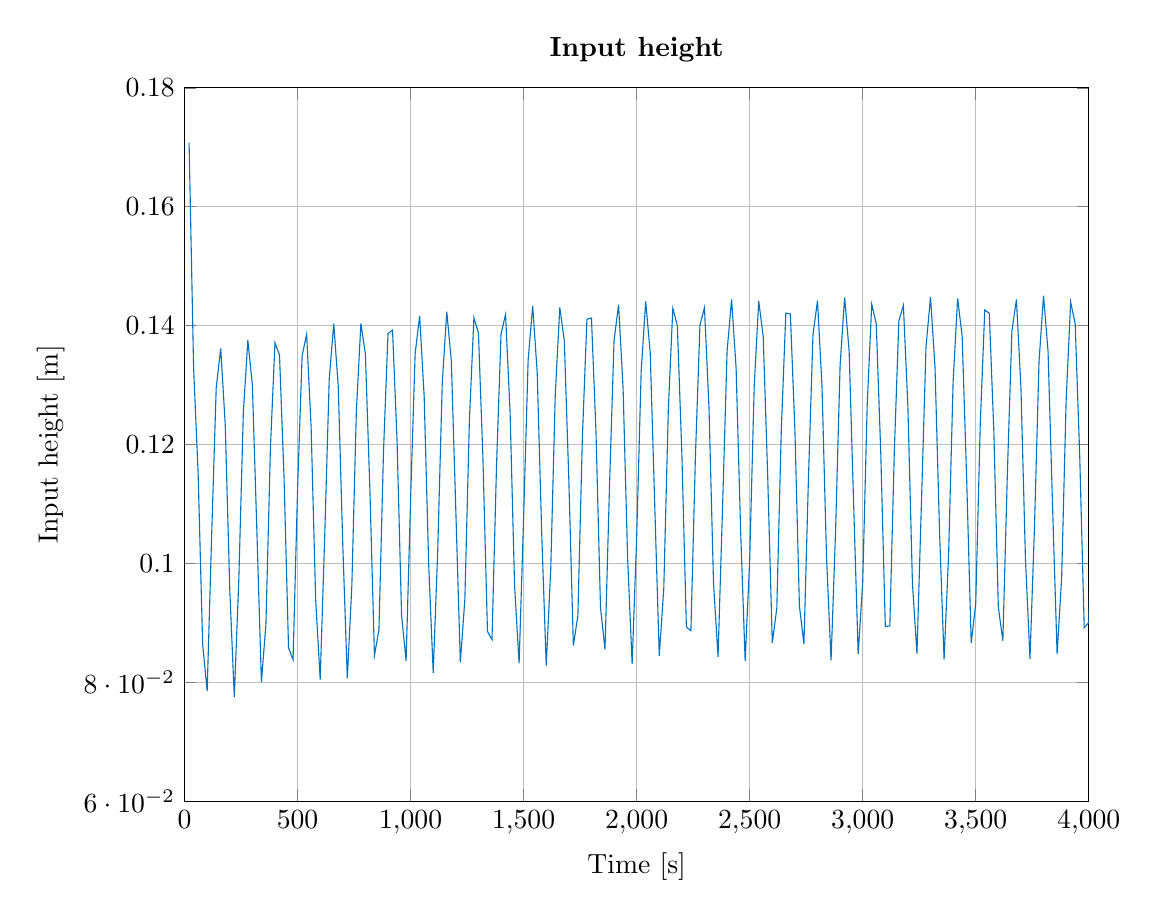
\begin{tikzpicture}

\begin{axis}[%
width=4.521in,
height=3.566in,
at={(0.758in,0.481in)},
scale only axis,
xmin=0,
xmax=4000,
xlabel={Time [s]},
xmajorgrids,
ymin=0.06,
ymax=0.18,
ylabel={Input height [m]},
ymajorgrids,
axis background/.style={fill=white},
title style={font=\bfseries},
title={Input height}
]
\addplot [color=mycolor1,solid,forget plot]
  table[row sep=crcr]{%
20	0.1708\\
40	0.132928350974997\\
60	0.115176105594743\\
80	0.0864513834981209\\
100	0.0785073041983677\\
120	0.104908900789824\\
140	0.12951180894696\\
160	0.136145849754549\\
180	0.123304522282863\\
200	0.0956640893491112\\
220	0.0775040090607498\\
240	0.097241577189598\\
260	0.125361058446894\\
280	0.13753992465754\\
300	0.129963142533142\\
320	0.105334869701811\\
340	0.0800224437795125\\
360	0.0897893682556843\\
380	0.119612642427884\\
400	0.137111150712519\\
420	0.135070464693904\\
440	0.114554696952337\\
460	0.0857892711675269\\
480	0.0837791436020674\\
500	0.112511607815721\\
520	0.134903594474349\\
540	0.138552501507921\\
560	0.122771607244799\\
580	0.0938650095818788\\
600	0.0804564400669687\\
620	0.104474824752048\\
640	0.131007653427119\\
660	0.140334890017599\\
680	0.129712808586803\\
700	0.103036925371309\\
720	0.0806643971986958\\
740	0.0962215572449868\\
760	0.125549849739593\\
780	0.140370154672904\\
800	0.135240760401737\\
820	0.112226779208414\\
840	0.0844987486889936\\
860	0.0888285824585309\\
880	0.118701158744187\\
900	0.138663651200875\\
920	0.139250759436304\\
940	0.120705150306368\\
960	0.0912714118079881\\
980	0.083579405531876\\
1000	0.110742251496598\\
1020	0.135278795221285\\
1040	0.141641388286449\\
1060	0.128076985749285\\
1080	0.0998135374168822\\
1100	0.0815855928894455\\
1120	0.102192024378863\\
1140	0.130322540235795\\
1160	0.14233318969531\\
1180	0.13414577981529\\
1200	0.108918171310388\\
1220	0.0833518054545054\\
1240	0.0939281869114499\\
1260	0.123933152975487\\
1280	0.141297541038796\\
1300	0.138784674034819\\
1320	0.117664450473044\\
1340	0.088557322335607\\
1360	0.087160353395477\\
1380	0.116309334447878\\
1400	0.138569937483976\\
1420	0.141877148530319\\
1440	0.125501310005549\\
1460	0.0962061662343507\\
1480	0.0831551233104718\\
1500	0.107811241006105\\
1520	0.134240189624114\\
1540	0.14332010750158\\
1560	0.132148145945986\\
1580	0.105042575786641\\
1600	0.0827868844892155\\
1620	0.0991059319544939\\
1640	0.128431275096959\\
1660	0.143052512211598\\
1680	0.137448603956136\\
1700	0.11396643774575\\
1720	0.0861672601599018\\
1740	0.0912420922173456\\
1760	0.121299045476906\\
1780	0.141077371271379\\
1800	0.141276061180672\\
1820	0.122239695591603\\
1840	0.0926011409544864\\
1860	0.0855097666724507\\
1880	0.113093945219898\\
1900	0.137461563812763\\
1920	0.143511643161814\\
1940	0.129460562084177\\
1960	0.100898653931902\\
1980	0.0830543176364308\\
2000	0.104294963133188\\
2020	0.132315636627854\\
2040	0.144065855789387\\
2060	0.135422370144798\\
2080	0.109830488155812\\
2100	0.0844206360774794\\
2120	0.0957449580867697\\
2140	0.125775486297432\\
2160	0.142906773608987\\
2180	0.139985820026014\\
2200	0.118458663481573\\
2220	0.0893144489261066\\
2240	0.0886409933526333\\
2260	0.118025976017169\\
2280	0.140071190162037\\
2300	0.143022998193802\\
2320	0.126220081071607\\
2340	0.0967442956495507\\
2360	0.0842677673763693\\
2380	0.109400445511703\\
2400	0.135652188199488\\
2420	0.144422635171875\\
2440	0.132824687996035\\
2460	0.105441732179539\\
2480	0.0835406706264177\\
2500	0.100532698292127\\
2520	0.129774461209446\\
2540	0.144119155297903\\
2560	0.138107732186833\\
2580	0.114287103781102\\
2600	0.0866153906305095\\
2620	0.0924464483101917\\
2640	0.122589225831493\\
2660	0.142114162986778\\
2680	0.141935096889593\\
2700	0.122524364289836\\
2720	0.0928246509626091\\
2740	0.0864308016721766\\
2760	0.114331427410344\\
2780	0.138475441800476\\
2800	0.144181658271494\\
2820	0.12973876910282\\
2840	0.100982517116477\\
2860	0.0836596880317458\\
2880	0.105453555269321\\
2900	0.133315262550935\\
2920	0.144753144166385\\
2940	0.135715343203513\\
2960	0.109845253989081\\
2980	0.0847251237769431\\
3000	0.0967693111955432\\
3020	0.126769012365953\\
3040	0.143614442703647\\
3060	0.140309255301374\\
3080	0.118453867398595\\
3100	0.0893769594857311\\
3120	0.0894596586718783\\
3140	0.119014131055227\\
3160	0.140800896796957\\
3180	0.143388179975495\\
3200	0.126227320150896\\
3220	0.0966466549655828\\
3240	0.0848203079879274\\
3260	0.110365780777073\\
3280	0.136405744069054\\
3300	0.144836733600069\\
3320	0.132864343923806\\
3340	0.105263236478811\\
3360	0.0838055366654276\\
3380	0.101430751111723\\
3400	0.130554120400097\\
3420	0.14458549396444\\
3440	0.138194441733443\\
3460	0.114088177744572\\
3480	0.0866217886188291\\
3500	0.0932080458827534\\
3520	0.123394541518732\\
3540	0.14263299041704\\
3560	0.142080257438338\\
3580	0.122343616375705\\
3600	0.092641365470617\\
3620	0.0869810135256635\\
3640	0.115151230325543\\
3660	0.139045337930991\\
3680	0.144393662862\\
3700	0.129598955425065\\
3720	0.10069199142982\\
3740	0.0839474316098852\\
3760	0.106255334541633\\
3780	0.133934534286908\\
3800	0.145036799695405\\
3820	0.135631053464026\\
3840	0.109519135359877\\
3860	0.084746853861714\\
3880	0.0974936694262138\\
3900	0.127435277239433\\
3920	0.143970738557916\\
3940	0.140291758239229\\
3960	0.118141454854766\\
3980	0.0891792886934057\\
4000	0.0900290525114048\\
4020	0.11971970341977\\
};
\end{axis}
\end{tikzpicture}%
% \caption{Input flow for the simulation.}
% \label{fig:height_input_for_comparision}
% \end{figure}

% In figure \ref{fig:height_output_nonlinear_and_linear_model} a comparison of the output nonlinear model and the linear model is shown.

% \begin{figure}[H]
%  \centering
%  % This file was created by matlab2tikz.
%
%The latest updates can be retrieved from
%  http://www.mathworks.com/matlabcentral/fileexchange/22022-matlab2tikz-matlab2tikz
%where you can also make suggestions and rate matlab2tikz.
%
\definecolor{mycolor1}{rgb}{0.00000,0.44700,0.74100}%
\definecolor{mycolor2}{rgb}{0.85000,0.32500,0.09800}%
%
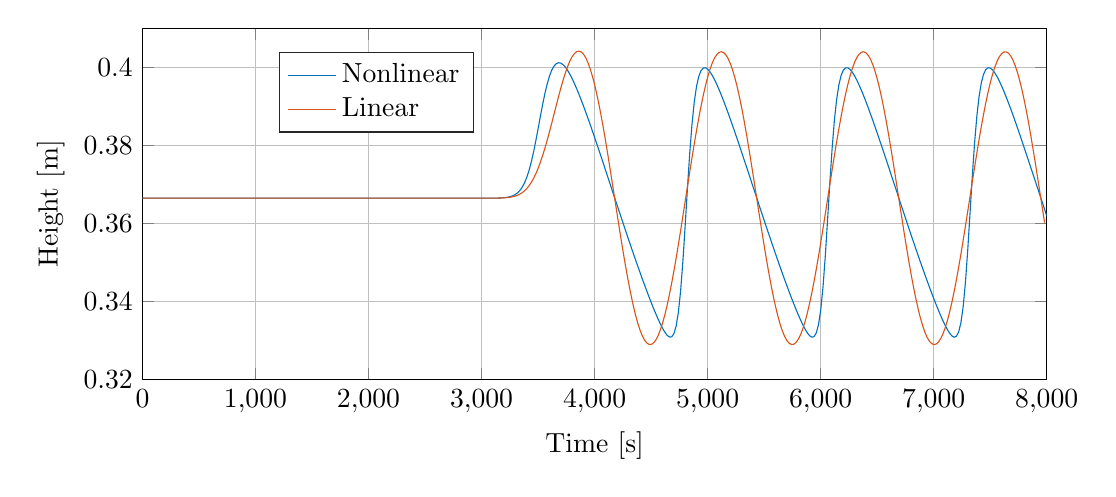
\begin{tikzpicture}

\begin{axis}[%
width=4.521in,
height=1.7566in,
at={(0.758in,0.481in)},
scale only axis,
xmin=1,
xmajorgrids,
ymajorgrids,
xmax=8000,
xlabel={Time [s]},
ymin=0.32,
ymax=0.41,
ylabel={Height [m]},
axis background/.style={fill=white},
legend style={at={(0.151,0.703)},anchor=south west,legend cell align=left,align=left,draw=white!15!black}
]
\addplot [color=mycolor1,solid]
  table[row sep=crcr]{%
1	0.366466627539343\\
21	0.366466665471691\\
41	0.366466692465574\\
61	0.366466711161801\\
81	0.366466723804557\\
101	0.366466732185832\\
121	0.36646673764237\\
141	0.366466741130459\\
161	0.366466743316878\\
181	0.366466744658372\\
201	0.366466745462716\\
221	0.366466745933408\\
241	0.366466746202002\\
261	0.366466746351381\\
281	0.366466746432328\\
301	0.366466746475058\\
321	0.366466746497021\\
341	0.366466746507986\\
361	0.366466746513251\\
381	0.366466746515595\\
401	0.366466746516464\\
421	0.366466746516784\\
441	0.366466746517842\\
461	0.366466746523015\\
481	0.366466746542095\\
501	0.366466746602594\\
521	0.366466746778925\\
541	0.366466747266689\\
561	0.366466748569185\\
581	0.366466751960835\\
601	0.366466760628919\\
621	0.366466782467414\\
641	0.366466824991748\\
661	0.366466877551302\\
681	0.366466909012503\\
701	0.366466897208555\\
721	0.366466852534906\\
741	0.366466804147601\\
761	0.366466772150041\\
781	0.366466758747709\\
801	0.366466757277496\\
821	0.366466761510951\\
841	0.366466768027839\\
861	0.366466774891905\\
881	0.366466780360355\\
901	0.366466782584759\\
921	0.366466779950668\\
941	0.366466771652426\\
961	0.366466758289697\\
981	0.366466742200663\\
1001	0.366466727015492\\
1021	0.366466716248985\\
1041	0.366466711712184\\
1061	0.36646671292079\\
1081	0.366466717849068\\
1101	0.366466724270585\\
1121	0.366466730692934\\
1141	0.366466736503687\\
1161	0.366466741612614\\
1181	0.366466746070639\\
1201	0.366466749918425\\
1221	0.366466753212207\\
1241	0.366466756057859\\
1261	0.366466758568098\\
1281	0.366466760782904\\
1301	0.366466762630246\\
1321	0.366466763956583\\
1341	0.366466764600551\\
1361	0.366466764466437\\
1381	0.366466763568626\\
1401	0.366466762037936\\
1421	0.366466760093622\\
1441	0.366466757992639\\
1461	0.366466755973411\\
1481	0.366466754212242\\
1501	0.366466752803997\\
1521	0.366466751767025\\
1541	0.366466751062805\\
1561	0.366466750618922\\
1581	0.366466750348598\\
1601	0.366466750165625\\
1621	0.366466749995936\\
1641	0.366466749786227\\
1661	0.3664667495087\\
1681	0.366466749160881\\
1701	0.366466748760672\\
1721	0.366466748338205\\
1741	0.366466747926767\\
1761	0.366466747555017\\
1781	0.366466747241989\\
1801	0.366466746995384\\
1821	0.366466746812749\\
1841	0.366466746684462\\
1861	0.366466746597258\\
1881	0.366466746537244\\
1901	0.366466746491858\\
1921	0.366466746450686\\
1941	0.366466746405459\\
1961	0.366466746349626\\
1981	0.366466746277887\\
2001	0.366466746185904\\
2021	0.366466746070288\\
2041	0.366466745928832\\
2061	0.366466745760932\\
2081	0.366466745568062\\
2101	0.366466745354198\\
2121	0.366466745126059\\
2141	0.366466744893064\\
2161	0.366466744666916\\
2181	0.366466744460798\\
2201	0.366466744288228\\
2221	0.366466744161677\\
2241	0.366466744091142\\
2261	0.366466744082878\\
2281	0.366466744138518\\
2301	0.366466744254728\\
2321	0.366466744423502\\
2341	0.36646674463305\\
2361	0.36646674486915\\
2381	0.366466745116762\\
2401	0.366466745361616\\
2421	0.366466745591559\\
2441	0.366466745797464\\
2461	0.366466745973624\\
2481	0.366466746117661\\
2501	0.366466746230052\\
2521	0.366466746313472\\
2541	0.366466746372187\\
2561	0.366466746411741\\
2581	0.366466746439263\\
2601	0.366466746464757\\
2621	0.366466746503873\\
2641	0.366466746582789\\
2661	0.366466746746095\\
2681	0.366466747069193\\
2701	0.36646674767828\\
2721	0.366466748783901\\
2741	0.366466750739029\\
2761	0.366466754138687\\
2781	0.366466759982299\\
2801	0.36646676991917\\
2821	0.366466786593398\\
2841	0.366466814088952\\
2861	0.36646685843496\\
2881	0.366466928083948\\
2901	0.366467034252727\\
2921	0.366467190986076\\
2941	0.366467414840061\\
2961	0.366467724280932\\
2981	0.366468138783252\\
3001	0.366468676751559\\
3021	0.366469356580593\\
3041	0.366470160960045\\
3061	0.366470781403547\\
3081	0.366471022304454\\
3101	0.366471811024978\\
3121	0.366476427538425\\
3141	0.366487208981108\\
3161	0.366506895988427\\
3181	0.366538154958313\\
3201	0.366586229651467\\
3221	0.366657715979119\\
3241	0.366763499523946\\
3261	0.366917391782519\\
3281	0.367139043129368\\
3301	0.367454993617361\\
3321	0.367897574460509\\
3341	0.36850855187551\\
3361	0.369337832554681\\
3381	0.37043866992242\\
3401	0.371865159415155\\
3421	0.373661877605495\\
3441	0.375850343116391\\
3461	0.378414236067563\\
3481	0.381291378533925\\
3501	0.384372804695217\\
3521	0.387512844594873\\
3541	0.3905512657543\\
3561	0.393339024106083\\
3581	0.395760573204265\\
3601	0.397742212920716\\
3621	0.399253919158054\\
3641	0.400302489298008\\
3661	0.400921093207355\\
3681	0.401154805407434\\
3701	0.401054639418849\\
3721	0.400670054854328\\
3741	0.400044850827336\\
3761	0.399219931578186\\
3781	0.398231007240009\\
3801	0.397106391211165\\
3821	0.395869603122493\\
3841	0.394540406299105\\
3861	0.393135051133942\\
3881	0.391665292279339\\
3901	0.390140640134986\\
3921	0.388569371321836\\
3941	0.386958604443187\\
3961	0.38531471749247\\
3981	0.383643494314967\\
4001	0.381950063243732\\
4021	0.380238783307623\\
4041	0.378513224443925\\
4061	0.376776293633958\\
4081	0.375030462811205\\
4101	0.373278012271646\\
4121	0.371521207603475\\
4141	0.369762211219868\\
4161	0.368003981050243\\
4181	0.366248027876198\\
4201	0.364495589895054\\
4221	0.36274817837337\\
4241	0.361007152561846\\
4261	0.359273873239861\\
4281	0.357549838340364\\
4301	0.355836692094989\\
4321	0.354136130444112\\
4341	0.352449809744458\\
4361	0.350779359466021\\
4381	0.349126509850378\\
4401	0.347493244675979\\
4421	0.345881887104931\\
4441	0.344295128405862\\
4461	0.342736107800051\\
4481	0.341208644935977\\
4501	0.339717633803796\\
4521	0.33826955870226\\
4541	0.336873179515492\\
4561	0.335540622633128\\
4581	0.334289313421881\\
4601	0.333145351925141\\
4621	0.332149220420964\\
4641	0.331364845137868\\
4661	0.330898154725945\\
4681	0.330920611138669\\
4701	0.331701861406759\\
4721	0.333627016627402\\
4741	0.337160391967049\\
4761	0.342687389504208\\
4781	0.350238925379372\\
4801	0.359278979022061\\
4821	0.368794883507088\\
4841	0.37768617476616\\
4861	0.385162896231032\\
4881	0.390901512494647\\
4901	0.394957571487544\\
4921	0.397587637909411\\
4941	0.399103627806496\\
4961	0.399788283600559\\
4981	0.399867543422794\\
5001	0.39950909035249\\
5021	0.398831004158808\\
5041	0.397918849649403\\
5061	0.396831762165564\\
5081	0.395610614486114\\
5101	0.394285153457823\\
5121	0.3928774871264\\
5141	0.391402867141369\\
5161	0.389872855411301\\
5181	0.388296811340508\\
5201	0.386682245098759\\
5221	0.385035455056554\\
5241	0.383361890492746\\
5261	0.381666299510196\\
5281	0.379952784260602\\
5301	0.378224870546435\\
5321	0.376485619899744\\
5341	0.374737747980308\\
5361	0.372983713654822\\
5381	0.371225798099233\\
5401	0.36946610982738\\
5421	0.367707346012034\\
5441	0.36595097244915\\
5461	0.364198476560114\\
5481	0.362451679502103\\
5501	0.360712151476488\\
5521	0.358981259374727\\
5541	0.357260283676455\\
5561	0.355550513137554\\
5581	0.353853314735917\\
5601	0.352170204157126\\
5621	0.350502906793907\\
5641	0.348853389344001\\
5661	0.347223875832671\\
5681	0.345616877505002\\
5701	0.344035250737081\\
5721	0.342482293026944\\
5741	0.340961912112083\\
5761	0.339478946792838\\
5781	0.338039744245102\\
5801	0.336653094188786\\
5821	0.335331662543733\\
5841	0.334094230460581\\
5861	0.332969329119605\\
5881	0.33200112977471\\
5901	0.331259545943237\\
5921	0.330859362295213\\
5941	0.330986746043631\\
5961	0.331929449934038\\
5981	0.334090502395966\\
6001	0.337936144363351\\
6021	0.343813694095991\\
6041	0.351668387281232\\
6061	0.360868048451852\\
6081	0.370353489513562\\
6101	0.37905274639098\\
6121	0.386250226872436\\
6141	0.391696415926776\\
6161	0.395492912117389\\
6181	0.39791438712643\\
6201	0.399272584189829\\
6221	0.399842045257527\\
6241	0.399838368584545\\
6261	0.399420391023125\\
6281	0.398698828491274\\
6301	0.397753915648429\\
6321	0.39664151960812\\
6341	0.395400219691452\\
6361	0.394058510709846\\
6381	0.392637268257605\\
6401	0.391151007525382\\
6421	0.389610922960775\\
6441	0.388026068082844\\
6461	0.386403786553424\\
6481	0.384750354678642\\
6501	0.383071309587512\\
6521	0.381371532327119\\
6541	0.37965522446482\\
6561	0.377925912612961\\
6581	0.37618653308801\\
6601	0.374439566745701\\
6621	0.372687159542499\\
6641	0.37093123369377\\
6661	0.369173762904317\\
6681	0.367417034013407\\
6701	0.365662198103127\\
6721	0.36391058042425\\
6741	0.362163892089778\\
6761	0.360423754996183\\
6781	0.358691793324237\\
6801	0.356969726303292\\
6821	0.355259390732162\\
6841	0.35356268781958\\
6861	0.351881499371196\\
6881	0.350217628278927\\
6901	0.348572810116784\\
6921	0.346948821893045\\
6941	0.345347668357579\\
6961	0.343771796843851\\
6981	0.342224323474826\\
7001	0.340709306127834\\
7021	0.339232116288827\\
7041	0.337799965520416\\
7061	0.336422693537365\\
7081	0.335114077562667\\
7101	0.333894157530986\\
7121	0.332793331053009\\
7141	0.331858832042384\\
7161	0.331166560746507\\
7181	0.330841014355229\\
7201	0.331083601276122\\
7221	0.332200931959585\\
7241	0.334612787291948\\
7261	0.33878182052881\\
7281	0.345008300801698\\
7301	0.353146585755168\\
7321	0.362473141745206\\
7341	0.371894864520334\\
7361	0.380379351083128\\
7381	0.387288734981073\\
7401	0.392443966115048\\
7421	0.395987436828022\\
7441	0.398207733177049\\
7461	0.399413773339763\\
7481	0.39987142748879\\
7501	0.399786479958598\\
7521	0.399309478906048\\
7541	0.398545717854504\\
7561	0.397571286774141\\
7581	0.396438242170758\\
7601	0.395181986798585\\
7621	0.393829305856599\\
7641	0.392398715789982\\
7661	0.390903890750215\\
7681	0.389355936704368\\
7701	0.387763859127099\\
7721	0.38613514005755\\
7741	0.384476100964206\\
7761	0.38279213085877\\
7781	0.381087856541197\\
7801	0.379367293514824\\
7821	0.37763396175543\\
7841	0.375890946504859\\
7861	0.374140924826797\\
7881	0.372386196920327\\
7901	0.370628746234173\\
7921	0.368870823401302\\
7941	0.367114475123368\\
7961	0.365360770569571\\
7981	0.363611061848541\\
8001	0.361866947544438\\
};
\addlegendentry{Nonlinear};

\addplot [color=mycolor2,solid]
  table[row sep=crcr]{%
1	0.366466627539343\\
21	0.366466627539343\\
41	0.366466627539343\\
61	0.366466627539343\\
81	0.366466627539343\\
101	0.366466627539343\\
121	0.366466627539343\\
141	0.366466627539343\\
161	0.366466627539343\\
181	0.366466627539343\\
201	0.366466627539343\\
221	0.366466627539343\\
241	0.366466627539343\\
261	0.366466627539343\\
281	0.366466627539343\\
301	0.366466627539343\\
321	0.366466627539343\\
341	0.366466627539343\\
361	0.366466627539343\\
381	0.366466627539343\\
401	0.366466627539343\\
421	0.366466627539343\\
441	0.366466627539343\\
461	0.366466627539343\\
481	0.366466627539343\\
501	0.366466627539343\\
521	0.366466627539343\\
541	0.366466627539343\\
561	0.366466627539343\\
581	0.366466627539343\\
601	0.366466627539343\\
621	0.366466627539343\\
641	0.366466627539343\\
661	0.366466627539343\\
681	0.366466627539343\\
701	0.366466627539343\\
721	0.366466627539343\\
741	0.366466627539343\\
761	0.366466627539343\\
781	0.366466627539343\\
801	0.366466627539343\\
821	0.366466627539343\\
841	0.366466627539343\\
861	0.366466627539343\\
881	0.366466627539343\\
901	0.366466627539343\\
921	0.366466627539343\\
941	0.366466627539343\\
961	0.366466627539343\\
981	0.366466627539343\\
1001	0.366466627539343\\
1021	0.366466627539343\\
1041	0.366466627539343\\
1061	0.366466627539343\\
1081	0.366466627539343\\
1101	0.366466627539343\\
1121	0.366466627539343\\
1141	0.366466627539343\\
1161	0.366466627539343\\
1181	0.366466627539343\\
1201	0.366466627539343\\
1221	0.366466627539343\\
1241	0.366466627539343\\
1261	0.366466627539343\\
1281	0.366466627539343\\
1301	0.366466627539343\\
1321	0.366466627539343\\
1341	0.366466627539343\\
1361	0.366466627539343\\
1381	0.366466627539343\\
1401	0.366466627539343\\
1421	0.366466627539343\\
1441	0.366466627539343\\
1461	0.366466627539343\\
1481	0.366466627539343\\
1501	0.366466627539343\\
1521	0.366466627539343\\
1541	0.366466627539343\\
1561	0.366466627539343\\
1581	0.366466627539343\\
1601	0.366466627539343\\
1621	0.366466627539343\\
1641	0.366466627539343\\
1661	0.366466627539343\\
1681	0.366466627539343\\
1701	0.366466627539343\\
1721	0.366466627539343\\
1741	0.366466627539343\\
1761	0.366466627539343\\
1781	0.366466627539343\\
1801	0.366466627539343\\
1821	0.366466627539343\\
1841	0.366466627539343\\
1861	0.366466627539343\\
1881	0.366466627539343\\
1901	0.366466627539343\\
1921	0.366466627539343\\
1941	0.366466627539343\\
1961	0.366466627539343\\
1981	0.366466627539343\\
2001	0.366466627539343\\
2021	0.366466627539343\\
2041	0.366466627539343\\
2061	0.366466627539343\\
2081	0.366466627539343\\
2101	0.366466627539343\\
2121	0.366466627539343\\
2141	0.366466627539343\\
2161	0.366466627539343\\
2181	0.366466627539343\\
2201	0.366466627539343\\
2221	0.366466627539343\\
2241	0.366466627539343\\
2261	0.366466627539343\\
2281	0.366466627539343\\
2301	0.366466627539343\\
2321	0.366466627539343\\
2341	0.366466627539343\\
2361	0.366466627539343\\
2381	0.366466627539343\\
2401	0.366466627539343\\
2421	0.366466627539343\\
2441	0.366466627539343\\
2461	0.366466627539343\\
2481	0.366466627539343\\
2501	0.366466627539344\\
2521	0.366466627539346\\
2541	0.366466627539352\\
2561	0.366466627539367\\
2581	0.366466627539406\\
2601	0.366466627539506\\
2621	0.366466627539753\\
2641	0.366466627540356\\
2661	0.366466627541801\\
2681	0.366466627545203\\
2701	0.36646662755307\\
2721	0.366466627570933\\
2741	0.366466627610775\\
2761	0.36646662769805\\
2781	0.366466627885832\\
2801	0.366466628282679\\
2821	0.366466629106458\\
2841	0.366466630786123\\
2861	0.366466634150207\\
2881	0.366466640768553\\
2901	0.366466653558754\\
2921	0.366466677839224\\
2941	0.366466723118069\\
2961	0.366466806064708\\
2981	0.36646695533534\\
3001	0.366467219229196\\
3021	0.366467677551623\\
3041	0.366468459553763\\
3061	0.366469770390096\\
3081	0.366471929138866\\
3101	0.366475421982078\\
3121	0.366480974508741\\
3141	0.366489647104487\\
3161	0.366502956796009\\
3181	0.366523027482528\\
3201	0.36655276798044\\
3221	0.366596073581188\\
3241	0.366658041875905\\
3261	0.366745187657059\\
3281	0.366865635273379\\
3301	0.36702926070058\\
3321	0.367247750875542\\
3341	0.367534545762865\\
3361	0.367904630390547\\
3381	0.368374150646985\\
3401	0.368959838382449\\
3421	0.369678247951269\\
3441	0.370544826519821\\
3461	0.371572862132087\\
3481	0.372772373883958\\
3501	0.374149024538009\\
3521	0.375703144660012\\
3541	0.377428956784265\\
3561	0.379314077344984\\
3581	0.38133935376884\\
3601	0.38347906633576\\
3621	0.385701492533075\\
3641	0.387969799702821\\
3661	0.390243203893882\\
3681	0.392478312407949\\
3701	0.394630556796896\\
3721	0.396655622738953\\
3741	0.398510792465058\\
3761	0.400156132117748\\
3781	0.401555477678416\\
3801	0.402677195711344\\
3821	0.403494716236732\\
3841	0.403986852338963\\
3861	0.404137933333533\\
3881	0.403937785095086\\
3901	0.403381592938361\\
3921	0.402469680258693\\
3941	0.401207231276515\\
3961	0.399603980007785\\
3981	0.397673881135668\\
4001	0.395434772626878\\
4021	0.392908035224715\\
4041	0.390118250560682\\
4061	0.387092857521657\\
4081	0.383861805500206\\
4101	0.380457202977927\\
4121	0.376912960270778\\
4141	0.373264425957107\\
4161	0.36954801732205\\
4181	0.365800845952344\\
4201	0.362060340322025\\
4221	0.358363867782038\\
4241	0.354748358794466\\
4261	0.351249936541774\\
4281	0.347903555208967\\
4301	0.344742650300615\\
4321	0.341798804333533\\
4341	0.339101431155141\\
4361	0.336677481990077\\
4381	0.334551176123472\\
4401	0.332743758896428\\
4421	0.331273289423679\\
4441	0.330154460150449\\
4461	0.329398450049507\\
4481	0.329012812924289\\
4501	0.329001401933752\\
4521	0.329364331092909\\
4541	0.330097974133665\\
4561	0.331195000737319\\
4581	0.332644449776703\\
4601	0.334431838836153\\
4621	0.336539308915026\\
4641	0.338945802868934\\
4661	0.341627275805773\\
4681	0.344556935334334\\
4701	0.347705509265027\\
4721	0.351041538087915\\
4741	0.354531689305745\\
4761	0.358141090481239\\
4781	0.361833677670961\\
4801	0.365572555764319\\
4821	0.369320367127311\\
4841	0.373039664867661\\
4861	0.376693286991785\\
4881	0.380244727715143\\
4901	0.383658502215979\\
4921	0.386900501187925\\
4941	0.389938331648914\\
4961	0.392741640601155\\
4981	0.395282418308246\\
5001	0.397535278159209\\
5021	0.399477710323108\\
5041	0.401090306659845\\
5061	0.402356954639877\\
5081	0.403264998335285\\
5101	0.403805364873624\\
5121	0.403972655091064\\
5141	0.403765197479053\\
5161	0.403185064885471\\
5181	0.402238053803429\\
5201	0.400933626454617\\
5221	0.399284816245919\\
5241	0.397308097543916\\
5261	0.395023221068461\\
5281	0.392453016550019\\
5301	0.38962316462254\\
5321	0.386561940231059\\
5341	0.38329993011779\\
5361	0.379869727209507\\
5381	0.376305604959795\\
5401	0.372643174900031\\
5421	0.368919030820735\\
5441	0.365170383138508\\
5461	0.361434687101853\\
5481	0.35774926855071\\
5501	0.354150950969006\\
5521	0.350675687556572\\
5541	0.347358201996655\\
5561	0.344231641508354\\
5581	0.341327245650566\\
5601	0.338674034186636\\
5621	0.336298517128476\\
5641	0.33422442985729\\
5661	0.33247249596749\\
5681	0.331060220203389\\
5701	0.330001713557588\\
5721	0.329307552278593\\
5741	0.328984672196448\\
5761	0.329036299422201\\
5781	0.329461918113679\\
5801	0.330257275629608\\
5821	0.331414425020598\\
5841	0.332921804432438\\
5861	0.334764352628319\\
5881	0.336923659475731\\
5901	0.339378149894427\\
5921	0.342103299427492\\
5941	0.345071879281605\\
5961	0.348254228388145\\
5981	0.351618549766786\\
6001	0.355131228230408\\
6021	0.35875716625694\\
6041	0.362460134672197\\
6061	0.366203134639811\\
6081	0.369948767341379\\
6101	0.373659607653087\\
6121	0.377298578085182\\
6141	0.380829319247989\\
6161	0.384216553142919\\
6181	0.387426435648562\\
6201	0.39042689467997\\
6221	0.39318795064232\\
6241	0.39568201597712\\
6261	0.397884170807974\\
6281	0.399772411931746\\
6301	0.401327872667297\\
6321	0.402535011365126\\
6341	0.40338176669439\\
6361	0.40385967815574\\
6381	0.40396397061583\\
6401	0.403693602018873\\
6421	0.403051273798518\\
6441	0.402043403886018\\
6461	0.40068006258438\\
6481	0.398974871949231\\
6501	0.396944869681735\\
6521	0.394610338893519\\
6541	0.391994605444527\\
6561	0.389123804878734\\
6581	0.386026621286432\\
6601	0.382734000702284\\
6621	0.37927884190277\\
6641	0.375695667692492\\
6661	0.372020279963719\\
6681	0.368289401975715\\
6701	0.364540311428072\\
6721	0.360810467994257\\
6741	0.357137139036939\\
6761	0.353557027244818\\
6781	0.350105903911493\\
6801	0.346818251520522\\
6821	0.343726919207841\\
6841	0.34086279454406\\
6861	0.338254494916066\\
6881	0.335928081591553\\
6901	0.333906799323449\\
6921	0.33221084409603\\
6941	0.33085716133332\\
6961	0.329859276586016\\
6981	0.329227160388656\\
7001	0.328967128637335\\
7021	0.329081779483356\\
7041	0.329569967373365\\
7061	0.330426814495338\\
7081	0.331643759516069\\
7101	0.333208643123178\\
7121	0.335105829516945\\
7141	0.337316362638051\\
7161	0.339818155570254\\
7181	0.342586211225559\\
7201	0.345592872106854\\
7221	0.348808096652485\\
7241	0.352199759401603\\
7261	0.355733971981154\\
7281	0.359375421707298\\
7301	0.363087724418075\\
7321	0.366833788011923\\
7341	0.370576183059695\\
7361	0.374277516787147\\
7381	0.377900806691172\\
7401	0.381409850056748\\
7421	0.384769585682503\\
7441	0.387946444200646\\
7461	0.390908683490992\\
7481	0.393626705837738\\
7501	0.396073353660056\\
7521	0.398224180861657\\
7541	0.400057697088114\\
7561	0.40155558245137\\
7581	0.402702870576012\\
7601	0.403488098138341\\
7621	0.403903419404116\\
7641	0.403944684620536\\
7661	0.403611481479199\\
7681	0.402907139235752\\
7701	0.401838695445065\\
7721	0.400416825644316\\
7741	0.398655736686546\\
7761	0.396573024790481\\
7781	0.394189499724935\\
7801	0.391528976884473\\
7821	0.388618039333867\\
7841	0.385485772198892\\
7861	0.382163472057373\\
7881	0.378684334234116\\
7901	0.375083121124203\\
7921	0.371395814858623\\
7941	0.367659257782722\\
7961	0.36391078433966\\
7981	0.360187848037\\
};
\addlegendentry{Linear};

\end{axis}
\end{tikzpicture}%
% \caption{Output height for the linear and Preissmann scheme simulation.}
% \label{fig:height_output_nonlinear_and_linear_model}
% \end{figure}
 


 %The fluctuations of the response of the nonlinear and linear are not identical as the top and bottom of the curves peaks at different times. However, the linear output looks very similar in phase as the input signal shown in figure \ref{fig:height_input_for_comparision} where the nonlinear has a faster response up going, and a slower one down going. It should be noted, that each time the response for both the models crosses the linearization point, they cross the same point. Hence it can be verified that the two models follows a similar pattern. It can be concluded that the plot of the nonlinear and linear responses are very similar, and therefore the linear model will be used to construct the MPC controller.  
In figure \ref{fig:linear_nonlinear_comparison_input_to_first_pipe} the input to the first pipe is shown. 

\begin{figure}[H]
 \centering
 % This file was created by matlab2tikz.
%
%The latest updates can be retrieved from
%  http://www.mathworks.com/matlabcentral/fileexchange/22022-matlab2tikz-matlab2tikz
%where you can also make suggestions and rate matlab2tikz.
%
\definecolor{mycolor1}{rgb}{0.00000,0.44700,0.74100}%
%
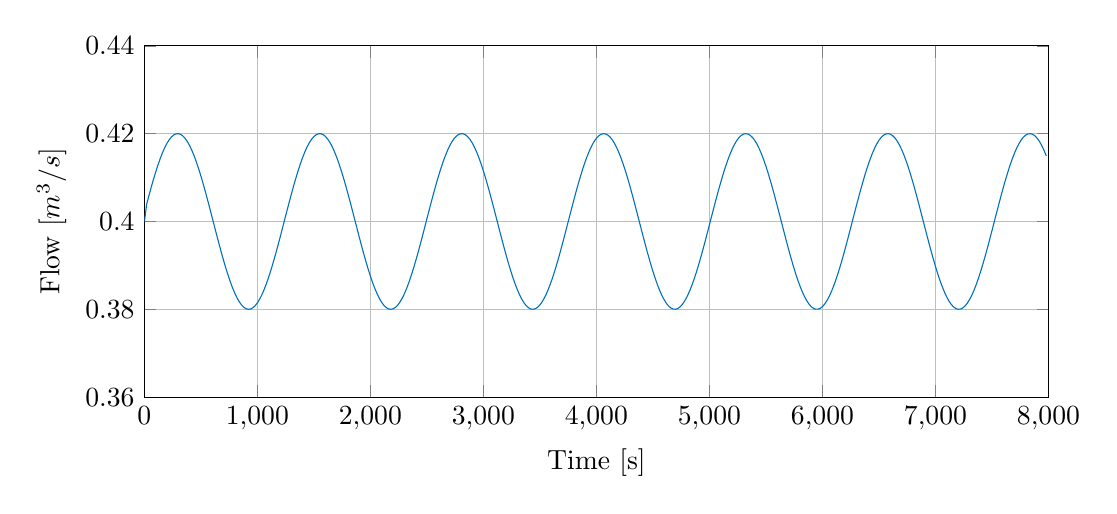
\begin{tikzpicture}

\begin{axis}[%
width=4.521in,
height=1.7566in,
at={(0.758in,0.481in)},
scale only axis,
xmin=0,
xmajorgrids,
ymajorgrids,
xmax=8000,
ymin=0.36,
ymax=0.44,
xlabel={Time [s]},
ylabel={Flow $[m^3/s]$},
axis background/.style={fill=white}
]
\addplot [color=mycolor1,solid,forget plot]
  table[row sep=crcr]{%
1	0.4\\
21	0.403973386615901\\
41	0.405910404133227\\
61	0.407788366846173\\
81	0.409588510772084\\
101	0.411292849467901\\
121	0.412884353744754\\
141	0.41434712181799\\
161	0.41566653819255\\
181	0.416829419696158\\
201	0.417824147201229\\
221	0.418640781719345\\
241	0.419271163708344\\
261	0.419708994599769\\
281	0.419949899732081\\
301	0.41999147206083\\
321	0.419833296209049\\
341	0.419476952617564\\
361	0.418926001753748\\
381	0.418185948536514\\
401	0.417264187332977\\
421	0.416169928076392\\
441	0.414914104243534\\
461	0.413509263611023\\
481	0.411969442882079\\
501	0.410310027436429\\
521	0.408547597604677\\
541	0.406699763003118\\
561	0.40478498658428\\
581	0.402822400161197\\
601	0.400831613248666\\
621	0.398832517131448\\
641	0.396845086117135\\
661	0.394889177959463\\
681	0.392984335446208\\
701	0.391149591134103\\
721	0.38940327718183\\
741	0.387762842181146\\
761	0.386244676816321\\
781	0.384863950093841\\
801	0.383634457778712\\
821	0.382568484551728\\
841	0.381676681265011\\
861	0.38096795852221\\
881	0.380449397646698\\
901	0.380126179927331\\
921	0.380001534848718\\
941	0.380076707823283\\
961	0.380350947747513\\
981	0.380821514506737\\
1001	0.381483706353445\\
1021	0.382330906885597\\
1041	0.383354651155522\\
1061	0.38454471024888\\
1081	0.385889193488592\\
1101	0.387374667242554\\
1121	0.388986289148047\\
1141	0.390707956411725\\
1161	0.392522466703395\\
1181	0.394411690036022\\
1201	0.396356749914558\\
1221	0.39833821194365\\
1241	0.400336278009687\\
1261	0.40233098409701\\
1281	0.404302399761756\\
1301	0.406230827270268\\
1321	0.408096998412332\\
1341	0.409882267022772\\
1361	0.411568795287764\\
1381	0.413139731974376\\
1401	0.414579380802518\\
1421	0.415873357276983\\
1441	0.417008732412571\\
1461	0.417974161916233\\
1481	0.418759999535495\\
1501	0.41935839344063\\
1521	0.41976336467754\\
1541	0.419970866907492\\
1561	0.419978826836795\\
1581	0.419787164932468\\
1601	0.419397796216902\\
1621	0.418814611133595\\
1641	0.418043436675126\\
1661	0.417091978161766\\
1681	0.41596974225247\\
1701	0.414687941957482\\
1721	0.413259384601644\\
1741	0.411698343857835\\
1761	0.410020417129158\\
1781	0.408242369704835\\
1801	0.406381967246987\\
1821	0.404457798282005\\
1841	0.402489088470141\\
1861	0.400495508509067\\
1881	0.398496977590764\\
1901	0.39651346437554\\
1921	0.394564787471781\\
1941	0.392670417414961\\
1961	0.390849282124494\\
1981	0.389119577782213\\
2001	0.387498587022142\\
2021	0.386002506248129\\
2041	0.384646283804728\\
2061	0.383443470618287\\
2081	0.382406084800567\\
2101	0.381544491567744\\
2121	0.380867299674596\\
2141	0.38038127539867\\
2161	0.380091274933872\\
2181	0.380000195868986\\
2201	0.38010894823592\\
2221	0.380416445416974\\
2241	0.380919615001958\\
2261	0.381613429486707\\
2281	0.382490956506231\\
2301	0.383543428100626\\
2321	0.384760328321619\\
2341	0.386129498304458\\
2361	0.387637257755259\\
2381	0.389268541639991\\
2401	0.391007050709308\\
2421	0.392835414355263\\
2441	0.394735364172684\\
2461	0.396687916491034\\
2481	0.398673562052976\\
2501	0.400672460944423\\
2521	0.402664640828399\\
2541	0.404630196502031\\
2561	0.406549488782754\\
2581	0.408403340736533\\
2601	0.410173229287447\\
2621	0.411841470294144\\
2641	0.413391395243932\\
2661	0.414807517799049\\
2681	0.416075688531032\\
2701	0.41718323629713\\
2721	0.418119094846169\\
2741	0.418873913388882\\
2761	0.4194401500279\\
2781	0.419812147113897\\
2801	0.419986187774958\\
2821	0.419960533054327\\
2841	0.419735439285492\\
2861	0.419313155530986\\
2881	0.418697901110494\\
2901	0.41789582344281\\
2921	0.416914936622859\\
2941	0.415765041347506\\
2961	0.41445762699024\\
2981	0.413005756803142\\
3001	0.4114239373932\\
3021	0.409727973777076\\
3041	0.407934811462612\\
3061	0.406062367134914\\
3081	0.404129349638756\\
3101	0.402155073045989\\
3121	0.400159263675719\\
3141	0.398161862995446\\
3161	0.396182828372516\\
3181	0.394241933666699\\
3201	0.39235857165632\\
3221	0.390551560272031\\
3241	0.388838954574264\\
3261	0.387237866353041\\
3281	0.385764293152618\\
3301	0.384432958429314\\
3321	0.383257164439605\\
3341	0.38224865932837\\
3361	0.381417519745313\\
3381	0.380772050162409\\
3401	0.380318699898367\\
3421	0.380061998679168\\
3441	0.38000451137854\\
3461	0.380146812390587\\
3481	0.380487479890637\\
3501	0.381023110041638\\
3521	0.381748351004176\\
3541	0.382655956410288\\
3561	0.38373685776677\\
3581	0.384980255064567\\
3601	0.38637372468889\\
3621	0.387903343551874\\
3641	0.389553828207465\\
3661	0.391308687558562\\
3681	0.393150387630608\\
3701	0.395060526765268\\
3721	0.397020019483716\\
3741	0.399009287182433\\
3761	0.401008453756136\\
3781	0.402997544193259\\
3801	0.404956684159659\\
3821	0.406866298576398\\
3841	0.408707307207458\\
3861	0.410461315303154\\
3881	0.412110797394392\\
3901	0.413639272401363\\
3921	0.415031468307043\\
3941	0.416273474750142\\
3961	0.417352882012833\\
3981	0.418258905014553\\
4001	0.418982491072958\\
4021	0.41951641035534\\
4041	0.419855328116718\\
4061	0.419995858002853\\
4081	0.419936595885576\\
4101	0.419678133892372\\
4121	0.419223054490042\\
4141	0.418575904681545\\
4161	0.417743150573847\\
4181	0.416733112770721\\
4201	0.415555883236022\\
4221	0.41422322445812\\
4241	0.412748451923005\\
4261	0.411146301070353\\
4281	0.409432780061884\\
4301	0.407625009833099\\
4321	0.405741053026555\\
4341	0.403799733515909\\
4361	0.401820448323997\\
4381	0.399822973814192\\
4401	0.397827268091518\\
4421	0.395853271587865\\
4441	0.393920707823779\\
4461	0.392048886337571\\
4481	0.39025650975079\\
4501	0.388561486897809\\
4521	0.386980753886675\\
4541	0.385530104879115\\
4561	0.384224034280492\\
4581	0.383075591916497\\
4601	0.382096252643606\\
4621	0.381295801696109\\
4641	0.380682236915279\\
4661	0.380261688837587\\
4681	0.380038359440412\\
4701	0.380014480157267\\
4721	0.380190289582057\\
4741	0.380564031085123\\
4761	0.381131970364909\\
4781	0.381888432759868\\
4801	0.382825859947801\\
4821	0.383934885466121\\
4841	0.385204428298442\\
4861	0.38662180359244\\
4881	0.388172849402698\\
4901	0.389842068192188\\
4921	0.391612781678535\\
4941	0.393467297477906\\
4961	0.395387085881452\\
4981	0.397352964998045\\
5001	0.399345292413383\\
5021	0.40134416145051\\
5041	0.403329600070743\\
5061	0.405281770427689\\
5081	0.407181167080443\\
5101	0.409008811885508\\
5121	0.410746443620129\\
5141	0.412376700442401\\
5161	0.413883293365045\\
5181	0.415251169009592\\
5201	0.416466660014762\\
5221	0.417517621596218\\
5241	0.41839355289324\\
5261	0.419085701889854\\
5281	0.419587152862078\\
5301	0.419892895477557\\
5321	0.41999987485714\\
5341	0.419907022098231\\
5361	0.419615264954903\\
5381	0.41912751856809\\
5401	0.418448656338462\\
5421	0.417585461233014\\
5441	0.416546558011908\\
5461	0.415342327052711\\
5481	0.413984800633102\\
5501	0.412487542708328\\
5521	0.410865513384645\\
5541	0.409134919442884\\
5561	0.407313052405652\\
5581	0.405418115766157\\
5601	0.403469043104918\\
5621	0.401485308911687\\
5641	0.399486734002789\\
5661	0.397493287478071\\
5681	0.395524887196264\\
5701	0.393601200762316\\
5721	0.391741449015189\\
5741	0.389964213979589\\
5761	0.388287253200514\\
5781	0.386727322315741\\
5801	0.385300007639024\\
5821	0.384019570426808\\
5841	0.382898804384459\\
5861	0.381948907835796\\
5881	0.381179371833141\\
5901	0.380597885325856\\
5921	0.380210258334909\\
5941	0.380020363901061\\
5961	0.380030099386724\\
5981	0.380239367518143\\
6001	0.380646077357324\\
6021	0.381246165193994\\
6041	0.382033635148853\\
6061	0.383000619082413\\
6081	0.384137455210854\\
6101	0.385432784643368\\
6121	0.386873664876444\\
6141	0.388445699111085\\
6161	0.390133180100864\\
6181	0.391919247093539\\
6201	0.393786054298113\\
6221	0.395714949194082\\
6241	0.397686658901255\\
6261	0.399681482747998\\
6281	0.401679489113835\\
6301	0.403660714579612\\
6321	0.40560536339538\\
6341	0.407494005272989\\
6361	0.409307769527099\\
6381	0.411028533624834\\
6401	0.412639104260138\\
6421	0.414123389143607\\
6441	0.415466557791324\\
6461	0.416655189706156\\
6481	0.417677408470917\\
6501	0.418523000413611\\
6521	0.419183516659062\\
6541	0.419652357547283\\
6561	0.419924838575097\\
6581	0.419998237202145\\
6601	0.419871820053608\\
6621	0.419546850247845\\
6641	0.419026574775736\\
6661	0.418316192057816\\
6681	0.417422800003384\\
6701	0.416355325090529\\
6721	0.415124433175721\\
6741	0.413742422924095\\
6761	0.412223102925252\\
6781	0.410581653722401\\
6801	0.408834476133384\\
6821	0.406999027379133\\
6841	0.405093646656881\\
6861	0.403137371900968\\
6881	0.401149749562099\\
6901	0.399150639305661\\
6921	0.39716001558052\\
6941	0.395197768040925\\
6961	0.393283502815657\\
6981	0.391436346610077\\
7001	0.389674755598401\\
7021	0.388016331015715\\
7041	0.386477643292245\\
7061	0.385074066487102\\
7081	0.383819624675762\\
7101	0.382726851826141\\
7121	0.381806666563329\\
7141	0.381068263074301\\
7161	0.380519019242633\\
7181	0.380164422931138\\
7201	0.380008017148944\\
7221	0.380051364650927\\
7241	0.380294032323176\\
7261	0.380733595510525\\
7281	0.381365662242906\\
7301	0.382183917118463\\
7321	0.383180184404958\\
7341	0.384344509728987\\
7361	0.385665259536787\\
7381	0.38712923733286\\
7401	0.388721815534995\\
7421	0.390427081628232\\
7441	0.392227997157453\\
7461	0.394106567969995\\
7481	0.396044024007271\\
7501	0.398021006848994\\
7521	0.400017763136114\\
7541	0.40201434193985\\
7561	0.403990794104776\\
7581	0.405927371574188\\
7601	0.407804724706159\\
7621	0.409604095608765\\
7641	0.41130750556274\\
7661	0.412897934658897\\
7681	0.414359491855433\\
7701	0.415677573755966\\
7721	0.416839010521846\\
7741	0.417832197460829\\
7761	0.418647210977324\\
7781	0.419275907725682\\
7801	0.419712005975813\\
7821	0.419951148378156\\
7841	0.419990945500878\\
7861	0.419830999704283\\
7881	0.4194729091139\\
7901	0.418920251652538\\
7921	0.418178549290868\\
7941	0.417255212873714\\
7961	0.41615946807334\\
7981	0.414902263209587\\
};
\end{axis}
\end{tikzpicture}%
\caption{Input flow to the first pipe.}
\label{fig:linear_nonlinear_comparison_input_to_first_pipe}
\end{figure}
The input to the sewer network is a sinusoidal. This is used to investigate if the nonlinear and linear model have a similar response for small perturbations. 
In the following figures comparisons are made between the nonlinear and linear model at different places in the sewer network. In figure \ref{fig:linear_nonlinear_comparison_input_first_pipe_into_tank} the output of the first pipe is shown.

\begin{figure}[H]
 \centering
 % This file was created by matlab2tikz.
%
%The latest updates can be retrieved from
%  http://www.mathworks.com/matlabcentral/fileexchange/22022-matlab2tikz-matlab2tikz
%where you can also make suggestions and rate matlab2tikz.
%
\definecolor{mycolor1}{rgb}{0.00000,0.44700,0.74100}%
\definecolor{mycolor2}{rgb}{0.85000,0.32500,0.09800}%
%
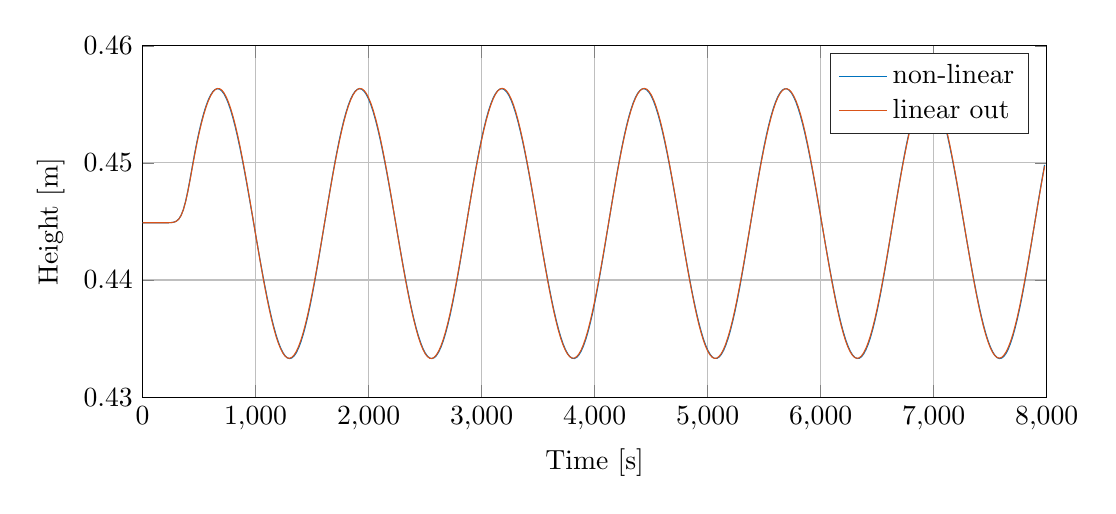
\begin{tikzpicture}

\begin{axis}[%
width=4.521in,
height=1.7566in,
at={(0.758in,0.481in)},
scale only axis,
xmin=0,
xmax=8000,
xlabel={Time [s]},
xmajorgrids,
ymin=0.43,
ymax=0.46,
ylabel={Height [m]},
ymajorgrids,
axis background/.style={fill=white},
legend style={legend cell align=left,align=left,draw=white!15!black}
]
\addplot [color=mycolor1,solid]
  table[row sep=crcr]{%
1	0.444890389772348\\
21	0.444890513105407\\
41	0.444890506028277\\
61	0.444890483539142\\
81	0.444890480180384\\
101	0.444890484549755\\
121	0.444890486153938\\
141	0.444890488187149\\
161	0.444890504664314\\
181	0.444890592226957\\
201	0.444890982364645\\
221	0.444892484368095\\
241	0.444897513208079\\
261	0.444912247332715\\
281	0.44495021707324\\
301	0.445036612933934\\
321	0.445210720248507\\
341	0.445522251378143\\
361	0.446018349496678\\
381	0.446723435380787\\
401	0.447621701901021\\
421	0.448655079484728\\
441	0.449741835128255\\
461	0.450806031355439\\
481	0.451799144263548\\
501	0.452702070386736\\
521	0.453512121631284\\
541	0.454229026870217\\
561	0.454849176245437\\
581	0.455366945609026\\
601	0.455777383168636\\
621	0.456077162609621\\
641	0.4562642983716\\
661	0.456337822034991\\
681	0.456297711358788\\
701	0.456144901035072\\
721	0.455881324013118\\
741	0.45550999835959\\
761	0.455035099955435\\
781	0.454461930626688\\
801	0.453796747739217\\
821	0.453046502054425\\
841	0.45221860533919\\
861	0.451320860272442\\
881	0.450361580453185\\
901	0.449349765856936\\
921	0.448295129482088\\
941	0.447207881921158\\
961	0.446098387500628\\
981	0.444976920226752\\
1001	0.443853654546849\\
1021	0.442738804741204\\
1041	0.441642695684339\\
1061	0.440575643739362\\
1081	0.439547742855924\\
1101	0.438568744696583\\
1121	0.437648092235126\\
1141	0.43679497083553\\
1161	0.43601820621578\\
1181	0.43532600044429\\
1201	0.434725669743442\\
1221	0.4342235459283\\
1241	0.4338250443032\\
1261	0.433534762217795\\
1281	0.433356475973452\\
1301	0.43329301863983\\
1321	0.433346112128187\\
1341	0.433516233625523\\
1361	0.433802546534754\\
1381	0.434202884036726\\
1401	0.434713766141664\\
1421	0.435330440621841\\
1441	0.436046931824876\\
1461	0.436856080427625\\
1481	0.437749576972346\\
1501	0.438718024815561\\
1521	0.439751064744405\\
1541	0.440837550909304\\
1561	0.441965747435319\\
1581	0.44312353243093\\
1601	0.44429858610053\\
1621	0.445478495604206\\
1641	0.446650744483934\\
1661	0.447802704273979\\
1681	0.448921824831973\\
1701	0.449996055560665\\
1721	0.4510142665232\\
1741	0.451966400742813\\
1761	0.452843343360739\\
1781	0.453636741725098\\
1801	0.454338982376328\\
1821	0.454943320892678\\
1841	0.455444049229152\\
1861	0.45583664108534\\
1881	0.456117868954708\\
1901	0.45628584381726\\
1921	0.456339907639262\\
1941	0.456280416738802\\
1961	0.456108584295105\\
1981	0.455826519958659\\
2001	0.455437413203808\\
2021	0.454945645843403\\
2041	0.454356677044245\\
2061	0.453676774614264\\
2081	0.452912808260128\\
2101	0.45207222519866\\
2121	0.451163123107327\\
2141	0.450194260118633\\
2161	0.449174942483414\\
2181	0.44811484418761\\
2201	0.447023832622007\\
2221	0.445911859124028\\
2241	0.444788967984734\\
2261	0.443665413175901\\
2281	0.442551742791173\\
2301	0.441458683628702\\
2321	0.440396837076628\\
2341	0.439376400121379\\
2361	0.438407091047066\\
2381	0.437498222247314\\
2401	0.436658717323784\\
2421	0.435896975935086\\
2441	0.435220688656884\\
2461	0.434636758074629\\
2481	0.434151357704681\\
2501	0.433770013415332\\
2521	0.433497563745665\\
2541	0.433337954641688\\
2561	0.433293961205547\\
2581	0.433366992134949\\
2601	0.43355707061449\\
2621	0.433862936396884\\
2641	0.434282124787469\\
2661	0.434810945465905\\
2681	0.435444431662193\\
2701	0.43617637582906\\
2721	0.436999463577042\\
2741	0.437905401908063\\
2761	0.438884947780973\\
2781	0.439927855583771\\
2801	0.441022867959747\\
2821	0.442157888136448\\
2841	0.44332035413576\\
2861	0.444497644483452\\
2881	0.445677272673719\\
2901	0.446846817264341\\
2921	0.447993827883114\\
2941	0.449105989715532\\
2961	0.450171525047388\\
2981	0.451179518034144\\
3001	0.452119946390693\\
3021	0.452983565354992\\
3041	0.453761932016254\\
3061	0.454447607111244\\
3081	0.455034300734856\\
3101	0.455516816322962\\
3121	0.45589094136335\\
3141	0.456153501256189\\
3161	0.456302549998853\\
3181	0.456337470078301\\
3201	0.456258860204721\\
3221	0.456068325305178\\
3241	0.455768346667694\\
3261	0.455362278565751\\
3281	0.45485440754496\\
3301	0.454250007361666\\
3321	0.45355534317873\\
3341	0.452777577140993\\
3361	0.451924577136784\\
3381	0.451004716011715\\
3401	0.450026756406294\\
3421	0.448999829815477\\
3441	0.447933449197968\\
3461	0.446837505655131\\
3481	0.445722231080723\\
3501	0.444598110993818\\
3521	0.443475741110116\\
3541	0.442365662189676\\
3561	0.441278232670896\\
3581	0.440223567945634\\
3601	0.439211523488113\\
3621	0.4382516809443\\
3641	0.437353313421694\\
3661	0.436525324038582\\
3681	0.435776156910669\\
3701	0.435113684321954\\
3721	0.434545081150217\\
3741	0.434076700594065\\
3761	0.433713967049432\\
3781	0.433461299771415\\
3801	0.43332205932846\\
3821	0.433298483970778\\
3841	0.43339160537411\\
3861	0.433601203275144\\
3881	0.433925866878906\\
3901	0.434363112610843\\
3921	0.434909390152479\\
3941	0.435559887168259\\
3961	0.436308287029692\\
3981	0.437146763726363\\
4001	0.438066310690831\\
4021	0.439057172270449\\
4041	0.440109051996531\\
4061	0.441211023601883\\
4081	0.442351376476064\\
4101	0.443517656900371\\
4121	0.44469694396713\\
4141	0.44587621067233\\
4161	0.447042630409426\\
4181	0.448183798971271\\
4201	0.449287894733353\\
4221	0.450343772209478\\
4241	0.451340962422148\\
4261	0.452269602625495\\
4281	0.453120402536078\\
4301	0.453884762882528\\
4321	0.454555039967992\\
4341	0.455124808414372\\
4361	0.455588979396579\\
4381	0.45594377182804\\
4401	0.456186628545273\\
4421	0.456316130034204\\
4441	0.456331897545565\\
4461	0.456234504455661\\
4481	0.456025457191654\\
4501	0.455707261141933\\
4521	0.455283495683509\\
4541	0.454758805495101\\
4561	0.454138793130599\\
4581	0.453429877793618\\
4601	0.452639186379266\\
4621	0.451774488769081\\
4641	0.450844147136555\\
4661	0.449857052611935\\
4681	0.448822548890726\\
4701	0.447750354531074\\
4721	0.446650489496358\\
4741	0.445533204159083\\
4761	0.444408906206146\\
4781	0.443288079076946\\
4801	0.442181189540063\\
4821	0.441098592173128\\
4841	0.440050440118039\\
4861	0.439046604513022\\
4881	0.43809661193001\\
4901	0.437209620889085\\
4921	0.436394426400625\\
4941	0.435659415136744\\
4961	0.435012398196607\\
4981	0.434460373603032\\
5001	0.434009382256267\\
5021	0.433664546306504\\
5041	0.433430166698647\\
5061	0.433309665549796\\
5081	0.433305328813018\\
5101	0.433418048684095\\
5121	0.433647293420932\\
5141	0.433991304334968\\
5161	0.434447291276899\\
5181	0.435011426280477\\
5201	0.435678660309672\\
5221	0.436442559259856\\
5241	0.437295312830546\\
5261	0.438227911218341\\
5281	0.439230386019289\\
5301	0.440292019118528\\
5321	0.441401475310849\\
5341	0.442546869119737\\
5361	0.443715827299868\\
5381	0.444895624321073\\
5401	0.446073415529398\\
5421	0.44723650859691\\
5441	0.448372581816034\\
5461	0.4494698074843\\
5481	0.450516913953775\\
5501	0.451503252101814\\
5521	0.45241890788172\\
5541	0.45325485055538\\
5561	0.454003057177939\\
5581	0.454656545652859\\
5601	0.455209316282111\\
5621	0.455656304997964\\
5641	0.455993462669208\\
5661	0.456217944490704\\
5681	0.456328250591823\\
5701	0.456324194418633\\
5721	0.456206753756379\\
5741	0.455977956871013\\
5761	0.455640857919376\\
5781	0.455199505526764\\
5801	0.454658808484111\\
5821	0.454024347222584\\
5841	0.453302275182958\\
5861	0.452499384079538\\
5881	0.451623260048019\\
5901	0.450682375295549\\
5921	0.449685997895997\\
5941	0.44864392715887\\
5961	0.447566190689611\\
5981	0.446462867483056\\
6001	0.445344087389156\\
6021	0.444220103006486\\
6041	0.443101292827982\\
6061	0.441998058569844\\
6081	0.440920689716611\\
6101	0.439879268713924\\
6121	0.438883618708383\\
6141	0.437943260782962\\
6161	0.437067370539719\\
6181	0.43626473389083\\
6201	0.435543671049785\\
6221	0.434911892375139\\
6241	0.434376313377315\\
6261	0.433942915203357\\
6281	0.433616699978158\\
6301	0.433401688577103\\
6321	0.433300879715876\\
6341	0.433316163969826\\
6361	0.433448260201261\\
6381	0.433696706695268\\
6401	0.434059854804847\\
6421	0.434534804148331\\
6441	0.435117310247565\\
6461	0.435801762104087\\
6481	0.43658128132876\\
6501	0.437447886073496\\
6521	0.438392618921671\\
6541	0.439405600428723\\
6561	0.440476064024545\\
6581	0.44159245590656\\
6601	0.442742622536888\\
6621	0.44391403210206\\
6641	0.445093972517359\\
6661	0.446269728676726\\
6681	0.447428771187851\\
6701	0.448558944413128\\
6721	0.449648594632486\\
6741	0.450686607252914\\
6761	0.451662402884795\\
6781	0.452565994453769\\
6801	0.453388177752358\\
6821	0.454120817481971\\
6841	0.454757071840551\\
6861	0.45529139957069\\
6881	0.455719364511314\\
6901	0.456037441878985\\
6921	0.45624302761583\\
6941	0.456334639107451\\
6961	0.456312103665058\\
6981	0.456176544844025\\
7001	0.455930167693354\\
7021	0.455576019177898\\
7041	0.455117911194731\\
7061	0.45456053368971\\
7081	0.453909604311749\\
7101	0.453171871299326\\
7121	0.452354925454666\\
7141	0.451466941073417\\
7161	0.450516499874561\\
7181	0.449512555741565\\
7201	0.448464480350975\\
7221	0.447382082297668\\
7241	0.446275531548444\\
7261	0.445155203554153\\
7281	0.444031516685893\\
7301	0.442914828526448\\
7321	0.441815399099514\\
7341	0.440743382900382\\
7361	0.439708808122178\\
7381	0.438721521130904\\
7401	0.437791096483806\\
7421	0.436926735566352\\
7441	0.436137181049679\\
7461	0.435430638321118\\
7481	0.434814658664352\\
7501	0.434295972563723\\
7521	0.43388034494677\\
7541	0.43357254161557\\
7561	0.433376388998747\\
7581	0.433294799478034\\
7601	0.433329660691391\\
7621	0.43348163497173\\
7641	0.433750010424328\\
7661	0.434132694303121\\
7681	0.434626311484839\\
7701	0.43522630812367\\
7721	0.435926993220556\\
7741	0.436721527304349\\
7761	0.437601912680156\\
7781	0.438559027968592\\
7801	0.439582713148978\\
7821	0.440661902909348\\
7841	0.441784821064919\\
7861	0.442939223605337\\
7881	0.444112621327594\\
7901	0.445292424514473\\
7921	0.446466043431772\\
7941	0.44762102069906\\
7961	0.448745204484524\\
7981	0.449826906363641\\
};
\addlegendentry{non-linear};

\addplot [color=mycolor2,solid]
  table[row sep=crcr]{%
1	0.444890389772348\\
21	0.444890389772348\\
41	0.444890389772355\\
61	0.444890389772541\\
81	0.444890389775642\\
101	0.444890389813297\\
121	0.444890390166431\\
141	0.44489039282735\\
161	0.444890409374298\\
181	0.444890495928743\\
201	0.444890882184263\\
221	0.444892368492001\\
241	0.444897340675172\\
261	0.444911893247545\\
281	0.444949340904319\\
301	0.44503439180022\\
321	0.445205414918557\\
341	0.445510714985277\\
361	0.445995870223076\\
381	0.446684498615593\\
401	0.447561894496245\\
421	0.448573306806098\\
441	0.449641218576109\\
461	0.450692585322813\\
481	0.451679254386228\\
501	0.452580798547114\\
521	0.453393290510725\\
541	0.454116297332662\\
561	0.454746840061463\\
581	0.455279930182363\\
601	0.45571071756884\\
621	0.456035253607315\\
641	0.456250200030005\\
661	0.456352672416096\\
681	0.456340573406984\\
701	0.456213160172925\\
721	0.455971535005333\\
741	0.455618799483335\\
761	0.45515971252297\\
781	0.454599949299955\\
801	0.453945342956883\\
821	0.453201578364317\\
841	0.452374582376141\\
861	0.451471384071542\\
881	0.450500800006038\\
901	0.449473331331564\\
921	0.448400238700667\\
941	0.447292450389352\\
961	0.446160123750598\\
981	0.445013118332286\\
1001	0.44386184447501\\
1021	0.442717678464867\\
1041	0.441592639255905\\
1061	0.440498753645289\\
1081	0.439447712939911\\
1101	0.438450907455252\\
1121	0.437519380091671\\
1141	0.436663333506031\\
1161	0.435891432538148\\
1181	0.435210522212488\\
1201	0.434626069440949\\
1221	0.434142971854945\\
1241	0.433766064000098\\
1261	0.433499961334761\\
1281	0.433348438577892\\
1301	0.433313815440262\\
1321	0.433396678049693\\
1341	0.433595951698165\\
1361	0.433909150494704\\
1381	0.434332631332846\\
1401	0.434861762799949\\
1421	0.435490983817437\\
1441	0.436213776026359\\
1461	0.437022636090526\\
1481	0.437909158163351\\
1501	0.438864254505488\\
1521	0.439878412722035\\
1541	0.440941855055084\\
1561	0.44204454319087\\
1581	0.443176031309829\\
1601	0.444325192717528\\
1621	0.445479974837789\\
1641	0.446627531238155\\
1661	0.447754983111103\\
1681	0.448850523365615\\
1701	0.449904084936619\\
1721	0.450907008237591\\
1741	0.451850985659383\\
1761	0.452727184259677\\
1781	0.453526214942013\\
1801	0.454238849847286\\
1821	0.45485690928054\\
1841	0.455373861441494\\
1861	0.455785006851037\\
1881	0.456087262442958\\
1901	0.456278621190341\\
1921	0.456357564453472\\
1941	0.456322877622462\\
1961	0.456174106107906\\
1981	0.455912331247259\\
2001	0.455540583049257\\
2021	0.455063487105873\\
2041	0.454486452706317\\
2061	0.453815125813193\\
2081	0.453055509464345\\
2101	0.452214460589447\\
2121	0.451299964236782\\
2141	0.450320923055998\\
2161	0.449286713619769\\
2181	0.448206924701535\\
2201	0.447091489060797\\
2221	0.445951121865542\\
2241	0.444797724984979\\
2261	0.443644298933781\\
2281	0.442504145172276\\
2301	0.441389737591078\\
2321	0.440312036866763\\
2341	0.439280667004367\\
2361	0.438304573262537\\
2381	0.437392442262983\\
2401	0.436552635745777\\
2421	0.435793017524897\\
2441	0.435121078309168\\
2461	0.434544246875923\\
2481	0.434069899525867\\
2501	0.433704773018557\\
2521	0.433454025600115\\
2541	0.433320543589112\\
2561	0.43330494418192\\
2581	0.433406207064533\\
2601	0.433622416192967\\
2621	0.433951102488997\\
2641	0.434389123975417\\
2661	0.434932432007858\\
2681	0.435576026002163\\
2701	0.436314019488222\\
2721	0.437139535721691\\
2741	0.43804436585631\\
2761	0.439018682859556\\
2781	0.440051206592138\\
2801	0.44112993806782\\
2821	0.442243114749561\\
2841	0.443379750237614\\
2861	0.444529353581211\\
2881	0.445681126644772\\
2901	0.446823486120229\\
2921	0.447944484294542\\
2941	0.449032772934579\\
2961	0.450078171365705\\
2981	0.451071367540379\\
3001	0.452003262307672\\
3021	0.452864779542292\\
3041	0.453647279525223\\
3061	0.454342976404003\\
3081	0.454944914025034\\
3101	0.455446785373219\\
3121	0.4558431226172\\
3141	0.456129820708517\\
3161	0.456304409041951\\
3181	0.456365718550462\\
3201	0.4563132878471\\
3221	0.456147125484542\\
3241	0.455868037016775\\
3261	0.455478200619014\\
3281	0.454981553680361\\
3301	0.454383759433077\\
3321	0.453691763735795\\
3341	0.452913152506017\\
3361	0.452055664033699\\
3381	0.451127140679669\\
3401	0.450135884568562\\
3421	0.449091092448642\\
3441	0.448003050116683\\
3461	0.446882979602266\\
3481	0.44574261536794\\
3501	0.444593679374753\\
3521	0.443447476072423\\
3541	0.442314790151107\\
3561	0.441206092115706\\
3581	0.440131856944932\\
3601	0.439102755052282\\
3621	0.438129594124355\\
3641	0.43722303695767\\
3661	0.43639319578276\\
3681	0.435649218593941\\
3701	0.434998971216242\\
3721	0.434448884065115\\
3741	0.434003978251915\\
3761	0.433668024214389\\
3781	0.433443733847404\\
3801	0.433332892833459\\
3821	0.433336439648007\\
3841	0.433454584757568\\
3861	0.43368695513527\\
3881	0.43403251264247\\
3901	0.434489012863003\\
3921	0.435052233236038\\
3941	0.435715660986231\\
3961	0.436471127205274\\
3981	0.437310017668234\\
4001	0.438224050840287\\
4021	0.439204960675942\\
4041	0.440243464751933\\
4061	0.441328554365713\\
4081	0.442447775256962\\
4101	0.443588259169498\\
4121	0.444737755132947\\
4141	0.445885124406248\\
4161	0.447020262022706\\
4181	0.448133675688588\\
4201	0.449215932667292\\
4221	0.450257128268015\\
4241	0.451246582625554\\
4261	0.452173022408881\\
4281	0.453025344850681\\
4301	0.453793684021933\\
4321	0.454470211166735\\
4341	0.455049242132673\\
4361	0.4555267185884\\
4381	0.455899499780252\\
4401	0.456164846041209\\
4421	0.456320210588378\\
4441	0.456363331119695\\
4461	0.456292614283769\\
4481	0.456107705679863\\
4501	0.45580995614096\\
4521	0.455402498863639\\
4541	0.454889925302644\\
4561	0.454277832057205\\
4581	0.453572531824893\\
4601	0.45278100638529\\
4621	0.451910976010202\\
4641	0.450970934685949\\
4661	0.449970102773578\\
4681	0.448918332141056\\
4701	0.447826000444342\\
4721	0.44670389708934\\
4741	0.445563088770344\\
4761	0.444414763684459\\
4781	0.44327007603731\\
4801	0.442140031297263\\
4821	0.441035446349169\\
4841	0.439966985264488\\
4861	0.438945238958777\\
4881	0.437980785021106\\
4901	0.437084107036913\\
4921	0.436265243643335\\
4941	0.435533219067545\\
4961	0.434895598650002\\
4981	0.434358533490799\\
5001	0.433927212845827\\
5021	0.433606163198563\\
5041	0.433398959830727\\
5061	0.43330761591402\\
5081	0.433332377727597\\
5101	0.433472270402486\\
5121	0.433725899717534\\
5141	0.434091682600257\\
5161	0.434567234043823\\
5181	0.435148460476103\\
5201	0.435829141493788\\
5221	0.436601281060684\\
5241	0.437455875517072\\
5261	0.438383550495247\\
5281	0.43937476870347\\
5301	0.440419660925055\\
5321	0.441507742774276\\
5341	0.442627809994805\\
5361	0.443768168629059\\
5381	0.444917107280183\\
5401	0.446063324470021\\
5421	0.447196059409817\\
5441	0.448304916492592\\
5461	0.449379602266665\\
5481	0.450409819419058\\
5501	0.451385399849604\\
5521	0.452296565857969\\
5541	0.4531341249766\\
5561	0.45388948344329\\
5581	0.45455456911198\\
5601	0.455121928467255\\
5621	0.455585181350023\\
5641	0.455939656748548\\
5661	0.456182737359074\\
5681	0.456313598363231\\
5701	0.456332538710274\\
5721	0.456240414089452\\
5741	0.456038452059906\\
5761	0.455728286991027\\
5781	0.455311958051419\\
5801	0.454791929926001\\
5821	0.454171429174161\\
5841	0.453455163049067\\
5861	0.452650025989175\\
5881	0.451765224268787\\
5901	0.450811577442015\\
5921	0.449800324268509\\
5941	0.448742122141311\\
5961	0.447646792705089\\
5981	0.44652381110037\\
6001	0.445383007980479\\
6021	0.444234912587969\\
6041	0.443090605131616\\
6061	0.441961380446626\\
6081	0.440858546536785\\
6101	0.43979339980387\\
6121	0.438777218419944\\
6141	0.437821144738154\\
6161	0.436935923899765\\
6181	0.436131507170986\\
6201	0.43541659496706\\
6221	0.434798318253311\\
6241	0.434282260360474\\
6261	0.433872786790388\\
6281	0.433573394711127\\
6301	0.433386828815816\\
6321	0.433314992660128\\
6341	0.433358848631911\\
6361	0.433518366377815\\
6381	0.433792400430412\\
6401	0.4341784526673\\
6421	0.434672506680569\\
6441	0.435269154706497\\
6461	0.435961973657106\\
6481	0.436743848362277\\
6501	0.437606996335097\\
6521	0.438542757359502\\
6541	0.439541442275503\\
6561	0.440592467984269\\
6581	0.441684734977051\\
6601	0.44280701185167\\
6621	0.443948149389292\\
6641	0.445097140862827\\
6661	0.4462431281786\\
6681	0.447375364177981\\
6701	0.448483071531797\\
6721	0.449555243075246\\
6741	0.450580597331544\\
6761	0.451547907607442\\
6781	0.452446692027122\\
6801	0.453267935462951\\
6821	0.454004369307012\\
6841	0.454650062950627\\
6861	0.455199611662303\\
6881	0.455647603513662\\
6901	0.455988859577583\\
6921	0.456219255520873\\
6941	0.456336401548036\\
6961	0.456339614800451\\
6981	0.456229298040232\\
7001	0.456006377709234\\
7021	0.455672366211776\\
7041	0.455230004707297\\
7061	0.45468388014889\\
7081	0.454040411235627\\
7101	0.453307155384608\\
7121	0.452491968712248\\
7141	0.451602623139969\\
7161	0.450647040355965\\
7181	0.449633797407583\\
7201	0.448572416995419\\
7221	0.447473216752157\\
7241	0.446346876955136\\
7261	0.445204080515105\\
7281	0.44405546477565\\
7301	0.442911840938643\\
7321	0.441784438559705\\
7341	0.440684953136637\\
7361	0.439625336459881\\
7381	0.438617419164376\\
7401	0.437672510752845\\
7421	0.436801075049601\\
7441	0.436012476150835\\
7461	0.435314751782642\\
7481	0.434714473802006\\
7501	0.434216857275746\\
7521	0.433826147403511\\
7541	0.433546002848166\\
7561	0.433379491193584\\
7581	0.43332864194775\\
7601	0.433393953146802\\
7621	0.433574307746083\\
7641	0.433867353469992\\
7661	0.434269979887886\\
7681	0.434778496510555\\
7701	0.435388424452672\\
7721	0.436094121551705\\
7741	0.436888531284432\\
7761	0.437763201810031\\
7781	0.438708542242743\\
7801	0.439714212812773\\
7821	0.440769553552586\\
7841	0.441863928180081\\
7861	0.442986832398122\\
7881	0.444127740346236\\
7901	0.445275883946775\\
7921	0.446420198881733\\
7941	0.44754945553792\\
7961	0.448652412826395\\
7981	0.44971790341445\\
};
\addlegendentry{linear out};

\end{axis}
\end{tikzpicture}%
\caption{Comparison of the nonlinear and linear model for the first pipe.}
\label{fig:linear_nonlinear_comparison_input_first_pipe_into_tank}
\end{figure}

It can be seen that the linear and nonlinear model for the output of the first pipe are identical, both in phase and amplitude as they follow each other throughout the simulation. In figure \ref{fig:linear_nonlinear_comparison_tank_height} the height of the tank for the linear and nonlinear model is shown.   

\begin{figure}[H]
 \centering
 % This file was created by matlab2tikz.
%
%The latest updates can be retrieved from
%  http://www.mathworks.com/matlabcentral/fileexchange/22022-matlab2tikz-matlab2tikz
%where you can also make suggestions and rate matlab2tikz.
%
\definecolor{mycolor1}{rgb}{0.00000,0.44700,0.74100}%
\definecolor{mycolor2}{rgb}{0.85000,0.32500,0.09800}%
%
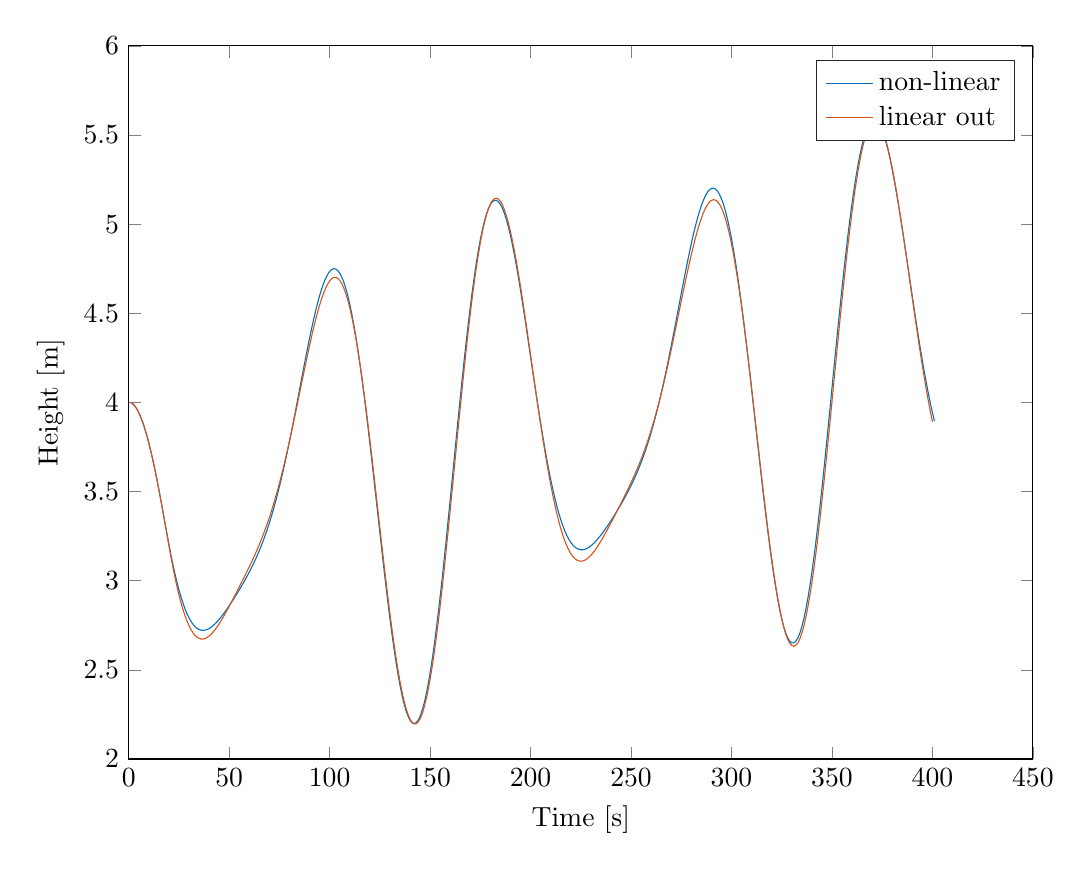
\begin{tikzpicture}

\begin{axis}[%
width=4.521in,
height=3.566in,
at={(0.758in,0.481in)},
scale only axis,
xmin=0,
xmax=450,
xlabel={Time [s]},
ymin=2,
ymax=6,
ylabel={Height [m]},
axis background/.style={fill=white},
legend style={legend cell align=left,align=left,draw=white!15!black}
]
\addplot [color=mycolor1,solid]
  table[row sep=crcr]{%
1	4\\
2	3.99281485388517\\
3	3.98089229877703\\
4	3.96429589132252\\
5	3.94311008270548\\
6	3.9174396709271\\
7	3.88740933874452\\
8	3.85316315177336\\
9	3.8148639575681\\
10	3.77269282398572\\
11	3.72684889042081\\
12	3.67755065665281\\
13	3.62504105449041\\
14	3.5696005464303\\
15	3.51157362705104\\
16	3.45141144588331\\
17	3.38972356923401\\
18	3.32731608105155\\
19	3.26518111636098\\
20	3.2044108927358\\
21	3.14604576423477\\
22	3.09091382444387\\
23	3.03953947939103\\
24	2.99216249068991\\
25	2.94883886540228\\
26	2.90955004501104\\
27	2.87426349888611\\
28	2.84294057056688\\
29	2.81552254385374\\
30	2.79192172269374\\
31	2.77202273780071\\
32	2.75568753538331\\
33	2.74275934933769\\
34	2.73306550701636\\
35	2.72642002404801\\
36	2.7226263004337\\
37	2.721480030925\\
38	2.72277250340294\\
39	2.72629422820897\\
40	2.73183850050269\\
41	2.73920436582854\\
42	2.74819864496649\\
43	2.75863713331165\\
44	2.77034559360359\\
45	2.78316126249621\\
46	2.79693507834779\\
47	2.81153406592424\\
48	2.82684296727721\\
49	2.84276464376228\\
50	2.85921963629096\\
51	2.87614577439579\\
52	2.89349839419222\\
53	2.9112509080306\\
54	2.92939501856447\\
55	2.94794023088455\\
56	2.96691302199623\\
57	2.98635624386529\\
58	3.00632882547801\\
59	3.02690520531904\\
60	3.04817389602818\\
61	3.07023519122016\\
62	3.09319861981231\\
63	3.11718075741643\\
64	3.14230349649008\\
65	3.16869239003441\\
66	3.19647461466528\\
67	3.22577637273701\\
68	3.25671984415372\\
69	3.2894199100356\\
70	3.32398082346616\\
71	3.36049293358475\\
72	3.39902953270337\\
73	3.43964384317141\\
74	3.48236609429393\\
75	3.52720065628709\\
76	3.57412333151374\\
77	3.62307902718105\\
78	3.67397999982163\\
79	3.72670475185107\\
80	3.78109761382962\\
81	3.83696896063655\\
82	3.89409575718629\\
83	3.95222200549035\\
84	4.01105910335552\\
85	4.07028686578493\\
86	4.12955608783606\\
87	4.1884926606673\\
88	4.24670223308934\\
89	4.30377434609423\\
90	4.35928584615839\\
91	4.41280416341873\\
92	4.46389102935742\\
93	4.51210677272424\\
94	4.55701510759308\\
95	4.59818829745396\\
96	4.63521239763498\\
97	4.6676920072518\\
98	4.69525411016837\\
99	4.71755122079759\\
100	4.73426458404141\\
101	4.74510796834544\\
102	4.74983177907082\\
103	4.74822662577377\\
104	4.74012575634822\\
105	4.72540659827193\\
106	4.70399209968418\\
107	4.67585224071647\\
108	4.64100547829182\\
109	4.59951966604376\\
110	4.55151220026104\\
111	4.49714942529824\\
112	4.4366455543213\\
113	4.37026156141339\\
114	4.29830445757568\\
115	4.22112683622518\\
116	4.1391259496082\\
117	4.05274162707454\\
118	3.96245314986437\\
119	3.86877586403452\\
120	3.77225809151969\\
121	3.67347814098661\\
122	3.5730408632071\\
123	3.47157357762109\\
124	3.36972177433085\\
125	3.26814510830234\\
126	3.16751377040952\\
127	3.06850479198893\\
128	2.97179767000619\\
129	2.87806904527067\\
130	2.78798673595144\\
131	2.70220377275245\\
132	2.62135287500041\\
133	2.54604127573687\\
134	2.47684551696406\\
135	2.41430610078412\\
136	2.35892230840736\\
137	2.31114754917323\\
138	2.27138521857775\\
139	2.2399846969867\\
140	2.21723718889125\\
141	2.20337156594245\\
142	2.19855089642627\\
143	2.20287042834939\\
144	2.2163571633426\\
145	2.23897024873761\\
146	2.27060120691742\\
147	2.31107391501639\\
148	2.36014531158305\\
149	2.41750773352706\\
150	2.48279260591013\\
151	2.55557438301653\\
152	2.6353741783311\\
153	2.72166360764023\\
154	2.81386951256678\\
155	2.91137934740276\\
156	3.01354645559838\\
157	3.11969502354505\\
158	3.22912531684563\\
159	3.3411197113053\\
160	3.4549491608404\\
161	3.56987928396506\\
162	3.68517568328921\\
163	3.8001087923494\\
164	3.91395871831499\\
165	4.02602030759564\\
166	4.1356084076647\\
167	4.24206311786446\\
168	4.34475464754931\\
169	4.44308740530391\\
170	4.5365032781363\\
171	4.62448442060915\\
172	4.70655590550318\\
173	4.78228835741548\\
174	4.85130050434096\\
175	4.91326151567244\\
176	4.96789293803832\\
177	5.01497001917251\\
178	5.05432234233896\\
179	5.08583391781238\\
180	5.10944298478154\\
181	5.12514169009504\\
182	5.13297565675503\\
183	5.13304336672014\\
184	5.12549526107344\\
185	5.11053245796529\\
186	5.08840500259912\\
187	5.05940960387706\\
188	5.02388686315411\\
189	4.98221805570749\\
190	4.93482157750421\\
191	4.88214913282223\\
192	4.82468161940369\\
193	4.76292462498394\\
194	4.69740367134432\\
195	4.62865958773718\\
196	4.55724421571929\\
197	4.48371602283685\\
198	4.40863487516368\\
199	4.33255578283922\\
200	4.25602249087664\\
201	4.17956215372525\\
202	4.10368148471851\\
203	4.02886356459552\\
204	3.95556421301237\\
205	3.88420768485663\\
206	3.81518243063442\\
207	3.74883781460426\\
208	3.68548213274398\\
209	3.62538175049055\\
210	3.56876106489736\\
211	3.51580307683372\\
212	3.46665033670343\\
213	3.42140592273802\\
214	3.38013419185734\\
215	3.34286144601899\\
216	3.3095770963077\\
217	3.28023588556642\\
218	3.25476117013109\\
219	3.23304871630656\\
220	3.21497045473843\\
221	3.20037797896109\\
222	3.18910577929613\\
223	3.18097416834297\\
224	3.17579192958097\\
225	3.17335895018597\\
226	3.1734691638205\\
227	3.17591383375378\\
228	3.18048485884105\\
229	3.18697772351799\\
230	3.19519396597629\\
231	3.20494328677988\\
232	3.21604546709222\\
233	3.22833215082569\\
234	3.24164844456063\\
235	3.25585428836781\\
236	3.2708255958748\\
237	3.28645518348848\\
238	3.30265350245163\\
239	3.31934917075966\\
240	3.3364892786261\\
241	3.35403943284029\\
242	3.37198353486955\\
243	3.39032332250237\\
244	3.40907771315782\\
245	3.42828202071983\\
246	3.44798719456635\\
247	3.46825918624809\\
248	3.48917826047491\\
249	3.51083779660073\\
250	3.53334232075012\\
251	3.55680511312319\\
252	3.58134605764457\\
253	3.60708994445857\\
254	3.63416463695315\\
255	3.66269835451624\\
256	3.69281605396968\\
257	3.72463573619848\\
258	3.75826549437987\\
259	3.79380128555438\\
260	3.83132466101574\\
261	3.87089978749623\\
262	3.91256981045269\\
263	3.95635318565508\\
264	4.00224059117054\\
265	4.05019265414474\\
266	4.10013837362758\\
267	4.15197395756877\\
268	4.20556183096076\\
269	4.26072980166597\\
270	4.31727066143945\\
271	4.37494259593204\\
272	4.43347055786761\\
273	4.4925484139359\\
274	4.55184151533162\\
275	4.61098946395128\\
276	4.6696090915148\\
277	4.72729782543722\\
278	4.7836375758674\\
279	4.83819905241586\\
280	4.8905461603198\\
281	4.94024012274361\\
282	4.98684336591363\\
283	5.02992364045296\\
284	5.06905878912138\\
285	5.10384197280769\\
286	5.13388669200904\\
287	5.15883115084216\\
288	5.1783420909747\\
289	5.19211843001435\\
290	5.19989467435589\\
291	5.20144371469021\\
292	5.19657879550007\\
293	5.18515500359067\\
294	5.16707089702465\\
295	5.14227061835941\\
296	5.11074624672515\\
297	5.07253970229527\\
298	5.02774355092192\\
299	4.976500576373\\
300	4.91900260892925\\
301	4.85548928570734\\
302	4.78624702339909\\
303	4.71160795367096\\
304	4.63194843592336\\
305	4.54768703916759\\
306	4.45928216013025\\
307	4.36722945041096\\
308	4.2720591009447\\
309	4.17433299360418\\
310	4.07464172866355\\
311	3.97360142104793\\
312	3.8718500232593\\
313	3.77004303368506\\
314	3.66884876671111\\
315	3.56894353856563\\
316	3.47100692881346\\
317	3.37571697028913\\
318	3.28374510092037\\
319	3.19575095190952\\
320	3.11237717351843\\
321	3.03424429733617\\
322	2.96194541348527\\
323	2.89604055127532\\
324	2.8370510171121\\
325	2.78545413186163\\
326	2.74167860754163\\
327	2.70610043102632\\
328	2.6790389815835\\
329	2.66075331665249\\
330	2.65143887375715\\
331	2.6512249248813\\
332	2.6601729231616\\
333	2.67827566834221\\
334	2.70545722671898\\
335	2.7415736611061\\
336	2.78641457950701\\
337	2.83970528597009\\
338	2.90110919557292\\
339	2.97023035897761\\
340	3.04661632586601\\
341	3.12976185098345\\
342	3.21911380386435\\
343	3.31407704707842\\
344	3.41402045105396\\
345	3.51828226495508\\
346	3.62617483767411\\
347	3.73698944557072\\
348	3.85000194650702\\
349	3.9644792001478\\
350	4.07968547733259\\
351	4.19488807684937\\
352	4.30936204696074\\
353	4.42239461749967\\
354	4.53329005553098\\
355	4.64137506844772\\
356	4.74600418794656\\
357	4.84656440006801\\
358	4.94247874646159\\
359	5.03320920737392\\
360	5.11825939471091\\
361	5.19717735497747\\
362	5.26955837603005\\
363	5.33504743694688\\
364	5.39334099831333\\
365	5.4441881103886\\
366	5.48739106335575\\
367	5.52280583289641\\
368	5.55034243023618\\
369	5.56996511018822\\
370	5.58169230986141\\
371	5.58559619318552\\
372	5.58180176312851\\
373	5.57048560428043\\
374	5.55187428444756\\
375	5.52624227519129\\
376	5.49390920767586\\
377	5.45523654501246\\
378	5.41062407828374\\
379	5.3605065875251\\
380	5.3053505303558\\
381	5.24565025018577\\
382	5.18192336124105\\
383	5.1147054943826\\
384	5.04454491654018\\
385	4.97199740362714\\
386	4.89762137691474\\
387	4.82197307044025\\
388	4.74560152687094\\
389	4.66904342647833\\
390	4.59281791356527\\
391	4.51742161190686\\
392	4.4433240170121\\
393	4.37096350522145\\
394	4.30074415787586\\
395	4.23303334381679\\
396	4.16815978792106\\
397	4.10641197774448\\
398	4.04803704469674\\
399	3.99324029031497\\
400	3.9421853164876\\
401	3.89499460281905\\
};
\addlegendentry{non-linear};

\addplot [color=mycolor2,solid]
  table[row sep=crcr]{%
1	4\\
2	3.99281440022489\\
3	3.98089141779219\\
4	3.96429466742038\\
5	3.94310852843827\\
6	3.91743776991418\\
7	3.88740708529663\\
8	3.85316053936219\\
9	3.81486093459038\\
10	3.77268912386595\\
11	3.72684337432509\\
12	3.67753913883185\\
13	3.62501024463012\\
14	3.56951382086477\\
15	3.51134312777761\\
16	3.45085350061734\\
17	3.38850389609367\\
18	3.32490689651401\\
19	3.26086469593234\\
20	3.19735754551971\\
21	3.13546001054403\\
22	3.07619581325621\\
23	3.02038619729244\\
24	2.96856310452994\\
25	2.92098453239321\\
26	2.87772649565134\\
27	2.83878562469752\\
28	2.80413966256706\\
29	2.77375918889231\\
30	2.74759670755254\\
31	2.72557777749333\\
32	2.70760023833348\\
33	2.69353634121097\\
34	2.68323383516125\\
35	2.67651651959424\\
36	2.67318610518368\\
37	2.67302626683397\\
38	2.67580860489385\\
39	2.68129925675633\\
40	2.68926430156763\\
41	2.69947246429996\\
42	2.71169505786083\\
43	2.72570486204734\\
44	2.74127655481244\\
45	2.758190461155\\
46	2.77623896485616\\
47	2.79523262762844\\
48	2.81500293195674\\
49	2.83540102240988\\
50	2.85629489650047\\
51	2.87756846491075\\
52	2.89912388894067\\
53	2.92088556786785\\
54	2.94280300432016\\
55	2.96485137684611\\
56	2.98703091082509\\
57	3.00936646239014\\
58	3.03190700860737\\
59	3.05472336566124\\
60	3.07790336305972\\
61	3.10154602873364\\
62	3.12575749555886\\
63	3.15065000183501\\
64	3.17634284530286\\
65	3.20296280112521\\
66	3.23064225139466\\
67	3.25951504816445\\
68	3.28971136351562\\
69	3.32135283865976\\
70	3.35454868962405\\
71	3.38939277948566\\
72	3.42596133177235\\
73	3.46431086503161\\
74	3.50447601865764\\
75	3.54646726337093\\
76	3.59026890339358\\
77	3.63583788243815\\
78	3.68310352483084\\
79	3.73196783839336\\
80	3.78230579374976\\
81	3.83396500514502\\
82	3.88676433312902\\
83	3.94049151036878\\
84	3.99490120017349\\
85	4.04971584458331\\
86	4.1046305830461\\
87	4.15932060281873\\
88	4.21344716263889\\
89	4.26665957414212\\
90	4.31859380658489\\
91	4.36887088799438\\
92	4.41709790756111\\
93	4.46287225353468\\
94	4.50578800782363\\
95	4.54544293830718\\
96	4.58144458644417\\
97	4.61341423281511\\
98	4.64098856354527\\
99	4.66382055133951\\
100	4.68158195460237\\
101	4.69396863639902\\
102	4.70070734279292\\
103	4.70156106983967\\
104	4.69633130076715\\
105	4.68485811011808\\
106	4.66702064224112\\
107	4.64273938010825\\
108	4.61197937354622\\
109	4.57475261278412\\
110	4.53111867734246\\
111	4.48118434790364\\
112	4.42510366270219\\
113	4.3630795742928\\
114	4.29536708433595\\
115	4.22227601516605\\
116	4.14417076185021\\
117	4.06146578977252\\
118	3.97461854542215\\
119	3.88412302122661\\
120	3.79050578668944\\
121	3.69432359996626\\
122	3.59616078158069\\
123	3.49662595586482\\
124	3.39634928376956\\
125	3.29598089223822\\
126	3.19618937416538\\
127	3.09765812683753\\
128	3.00107821425157\\
129	2.90713867994491\\
130	2.81651692743442\\
131	2.72987153220216\\
132	2.64783790317654\\
133	2.5710253008542\\
134	2.50001348075788\\
135	2.43534853860873\\
136	2.37753866771737\\
137	2.32705024922676\\
138	2.28430363838373\\
139	2.2496677582803\\
140	2.2234537120066\\
141	2.20590910720385\\
142	2.19721522934085\\
143	2.19748789352765\\
144	2.20678041583414\\
145	2.22508562613702\\
146	2.25233496368744\\
147	2.28839587223512\\
148	2.33307086495155\\
149	2.38610029478373\\
150	2.4471673430214\\
151	2.51590197071301\\
152	2.59188249129099\\
153	2.67463650867943\\
154	2.7636434802498\\
155	2.85833891581711\\
156	2.958118551448\\
157	3.06234190664612\\
158	3.17033661028885\\
159	3.28140474143919\\
160	3.3948302344061\\
161	3.50988507431779\\
162	3.62583329838828\\
163	3.74193413290112\\
164	3.85744637870939\\
165	3.97163497153952\\
166	4.08377900167909\\
167	4.19317961121229\\
168	4.29916622491028\\
169	4.40110036059106\\
170	4.49837759373784\\
171	4.59042931857685\\
172	4.67672581514473\\
173	4.75678091338381\\
174	4.8301573464424\\
175	4.89647148484589\\
176	4.95539642949017\\
177	5.00666307884176\\
178	5.05005961530232\\
179	5.08543054189667\\
180	5.1126764197232\\
181	5.1317547263438\\
182	5.14268135230373\\
183	5.14553179778543\\
184	5.14044122600704\\
185	5.12760290734496\\
186	5.10726502192496\\
187	5.07972617798186\\
188	5.04533026238728\\
189	5.00446129512958\\
190	4.95753878429585\\
191	4.90501370702604\\
192	4.84736489230623\\
193	4.78509560617983\\
194	4.71873049121387\\
195	4.64881295666393\\
196	4.57590217284673\\
197	4.50056794795699\\
198	4.42338262448818\\
199	4.34491172325763\\
200	4.26570688799794\\
201	4.18630329792636\\
202	4.10721992864316\\
203	4.02895855698105\\
204	3.95199883335327\\
205	3.87679063443408\\
206	3.80374741778049\\
207	3.73324340066727\\
208	3.66561456771732\\
209	3.60116150102129\\
210	3.54015188755756\\
211	3.48282142453608\\
212	3.42937263359204\\
213	3.37997167114148\\
214	3.33474399765706\\
215	3.2937707314359\\
216	3.25708787779384\\
217	3.22468957385159\\
218	3.1965343574163\\
219	3.1725518665718\\
220	3.15264762666721\\
221	3.13670521975603\\
222	3.12458656151609\\
223	3.11613144767592\\
224	3.11115749989987\\
225	3.10946161485236\\
226	3.11082361718534\\
227	3.11501173176686\\
228	3.12178841931948\\
229	3.1309150739812\\
230	3.1421551022387\\
231	3.15527600182056\\
232	3.17005135124518\\
233	3.18626314912038\\
234	3.2037043768516\\
235	3.22218147653031\\
236	3.24151656679536\\
237	3.26154935663942\\
238	3.28213872621155\\
239	3.30316389783505\\
240	3.32452511666079\\
241	3.34614384105002\\
242	3.36796259414572\\
243	3.38994475580475\\
244	3.41207457635342\\
245	3.43435757420532\\
246	3.45682123996896\\
247	3.47951551657257\\
248	3.50251203777455\\
249	3.52590130124138\\
250	3.54978824073636\\
251	3.57428802776176\\
252	3.59952362744324\\
253	3.625624528274\\
254	3.65272443625514\\
255	3.68095671801529\\
256	3.71044911073355\\
257	3.7413205085844\\
258	3.77368078022732\\
259	3.80763146790028\\
260	3.84326419708684\\
261	3.88065568918607\\
262	3.91986120300855\\
263	3.96090928549777\\
264	4.00379938910524\\
265	4.04850185780044\\
266	4.09495866567559\\
267	4.14308348860742\\
268	4.19276067453259\\
269	4.24384377647537\\
270	4.29615489914353\\
271	4.34948576206428\\
272	4.40360030578504\\
273	4.45823772372026\\
274	4.51311476615719\\
275	4.56792698393648\\
276	4.62234949702098\\
277	4.67603818144276\\
278	4.72863175213521\\
279	4.77975448997064\\
280	4.82901893025311\\
281	4.87602817095107\\
282	4.92037845227339\\
283	4.96166334842342\\
284	4.99948025008013\\
285	5.03343804471769\\
286	5.06316372222427\\
287	5.08830637759624\\
288	5.10853899315422\\
289	5.12355943533883\\
290	5.13309149249345\\
291	5.13688581717754\\
292	5.13472086083748\\
293	5.12640498792909\\
294	5.11178120763315\\
295	5.0907344805728\\
296	5.06319942169946\\
297	5.02916531532821\\
298	4.98867658795232\\
299	4.94182946966311\\
300	4.88876764871447\\
301	4.82967971438443\\
302	4.76479919195388\\
303	4.69440582897694\\
304	4.61882629787133\\
305	4.53843361290349\\
306	4.45364577375702\\
307	4.36492430478756\\
308	4.27277276432509\\
309	4.17773481406127\\
310	4.08039131534318\\
311	3.98135595117596\\
312	3.88126915388447\\
313	3.78079086369663\\
314	3.68059340135463\\
315	3.58135561607663\\
316	3.48375838843652\\
317	3.38848061716221\\
318	3.29619492786121\\
319	3.20756306607149\\
320	3.12323116120915\\
321	3.0438246002971\\
322	2.96994208360107\\
323	2.90214913581489\\
324	2.84097217388209\\
325	2.7868940691457\\
326	2.74035100857542\\
327	2.70172953772122\\
328	2.67136290511889\\
329	2.649526931844\\
330	2.63643648119307\\
331	2.6322434391256\\
332	2.63703623204657\\
333	2.65084024245426\\
334	2.67361854510173\\
335	2.70527275956482\\
336	2.74564385343696\\
337	2.79451250649017\\
338	2.85159881399067\\
339	2.91656190886006\\
340	2.98900090127534\\
341	3.06845848653744\\
342	3.15442733725718\\
343	3.24635761710874\\
344	3.3436630296927\\
345	3.44572388379015\\
346	3.55188821702711\\
347	3.66147387383335\\
348	3.77377371349836\\
349	3.88806341135564\\
350	4.00360919293304\\
351	4.11967326778472\\
352	4.235517179709\\
353	4.35040540902431\\
354	4.4636113984983\\
355	4.5744259000194\\
356	4.68216526811965\\
357	4.78617714678074\\
358	4.88584299178917\\
359	4.98057913735402\\
360	5.06983871503306\\
361	5.15311543798356\\
362	5.22994843693838\\
363	5.29992648767778\\
364	5.36269056814456\\
365	5.41793501103677\\
366	5.46540841658513\\
367	5.50491532472236\\
368	5.53631873616528\\
369	5.55954273946846\\
370	5.57457427509407\\
371	5.58146340342134\\
372	5.58032198896795\\
373	5.57132108096684\\
374	5.55468725231449\\
375	5.5306979976484\\
376	5.49967651581627\\
377	5.46198680804613\\
378	5.41803013333666\\
379	5.36824280717216\\
380	5.31309388842915\\
381	5.25308109499283\\
382	5.1887247748573\\
383	5.12056147131979\\
384	5.04913882264298\\
385	4.97501216300889\\
386	4.8987417055821\\
387	4.82088886078934\\
388	4.74201106822952\\
389	4.66265561022345\\
390	4.58335342431708\\
391	4.50461380895877\\
392	4.42692052917991\\
393	4.35072947163008\\
394	4.27646753590179\\
395	4.20453188365312\\
396	4.1352885687198\\
397	4.06907030219124\\
398	4.00617398347174\\
399	3.94685869728292\\
400	3.89134426856577\\
};
\addlegendentry{linear out};

\end{axis}
\end{tikzpicture}%
\caption{Comparison of the nonlinear and linear model for the tank. }
\label{fig:linear_nonlinear_comparison_tank_height}
\end{figure}
 
It is clear that the nonlinear and linear model for the tank are very similar as they only deviates a small amount at the peaks. In figure \ref{fig:linear_nonlinear_comparison_pipe_after_tank} the output of the pipe after the tank is shown.  

\begin{figure}[H]
 \centering
 % This file was created by matlab2tikz.
%
%The latest updates can be retrieved from
%  http://www.mathworks.com/matlabcentral/fileexchange/22022-matlab2tikz-matlab2tikz
%where you can also make suggestions and rate matlab2tikz.
%
\definecolor{mycolor1}{rgb}{0.00000,0.44700,0.74100}%
\definecolor{mycolor2}{rgb}{0.85000,0.32500,0.09800}%
%
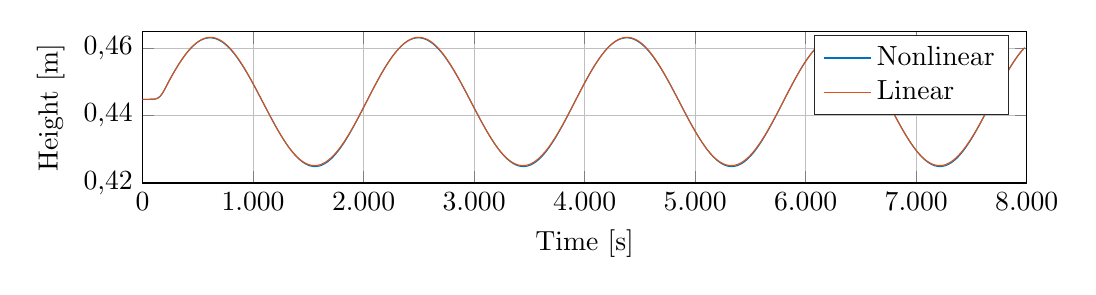
\begin{tikzpicture}

\begin{axis}[%
width=4.421in,
height=.7566in,
/pgf/number format/1000 sep={.},/pgf/number format/use comma,
at={(0.758in,0.481in)},
scale only axis,
xmin=0,
xmax=8000,
xlabel={Time [s]},
xmajorgrids,
ymin=0.42,
ymax=0.465,
ylabel={Height [m]},
ymajorgrids,
axis background/.style={fill=white},
legend style={legend cell align=left,align=left,draw=white!15!black}
]
\addplot [color=mycolor1,solid]
  table[row sep=crcr]{%
1	0.4448903921446\\
21	0.444890395604401\\
41	0.444890478989189\\
61	0.444891399462415\\
81	0.44489768087895\\
101	0.444927316973418\\
121	0.445029837966795\\
141	0.445299119740533\\
161	0.445848740544978\\
181	0.446737111169511\\
201	0.447900409457629\\
221	0.449181948114068\\
241	0.450445971436173\\
261	0.451649238232275\\
281	0.452805509195267\\
301	0.453923614919199\\
321	0.454996760490511\\
341	0.456018473924374\\
361	0.456985842499905\\
381	0.457895758609179\\
401	0.458744309155889\\
421	0.459526872446132\\
441	0.460238927080553\\
461	0.460877766766091\\
481	0.461442404335922\\
501	0.461931618263264\\
521	0.462343038226796\\
541	0.462673985796383\\
561	0.462922115566296\\
581	0.463085761808448\\
601	0.463165000862207\\
621	0.463161767963357\\
641	0.463077774152749\\
661	0.462912700515528\\
681	0.462665083217703\\
701	0.462334975525558\\
721	0.461925320066751\\
741	0.461439882474596\\
761	0.46088032121217\\
781	0.460247109256119\\
801	0.459542826148449\\
821	0.45877213118035\\
841	0.457938885851068\\
861	0.457045736413618\\
881	0.456096249484013\\
901	0.455095257701042\\
921	0.454047285512727\\
941	0.45295630118541\\
961	0.451826616747197\\
981	0.450662864559418\\
1001	0.449469684812144\\
1021	0.448252115056624\\
1041	0.447015762927058\\
1061	0.445766484480015\\
1081	0.444510082772652\\
1101	0.443251681187692\\
1121	0.441995298599495\\
1141	0.440745148396479\\
1161	0.439507469163443\\
1181	0.438289725378601\\
1201	0.437097776851792\\
1221	0.435935185912507\\
1241	0.434805514793038\\
1261	0.433713925442494\\
1281	0.432666274604885\\
1301	0.43166800385088\\
1321	0.430724234156608\\
1341	0.429839588257958\\
1361	0.429017425169056\\
1381	0.428260320657075\\
1401	0.427571617572048\\
1421	0.426955499857992\\
1441	0.426415400429793\\
1461	0.425953448340526\\
1481	0.425571672054113\\
1501	0.425272672419593\\
1521	0.425058857459238\\
1541	0.424931824128951\\
1561	0.424892442284851\\
1581	0.424940683805082\\
1601	0.425075517272546\\
1621	0.425295832195707\\
1641	0.425601309173907\\
1661	0.42599160714887\\
1681	0.426465142574227\\
1701	0.427019705714707\\
1721	0.427653493342147\\
1741	0.428363981002374\\
1761	0.42914653153053\\
1781	0.429995804679556\\
1801	0.430908099193119\\
1821	0.431881059821401\\
1841	0.432911394765246\\
1861	0.433993705632748\\
1881	0.435121373864266\\
1901	0.436288299080676\\
1921	0.437489773956437\\
1941	0.43872116706734\\
1961	0.439976132856488\\
1981	0.441247642314717\\
2001	0.442530281676256\\
2021	0.443819748072584\\
2041	0.445110556898724\\
2061	0.446395579129906\\
2081	0.447667614489687\\
2101	0.448920774822279\\
2121	0.450150357835776\\
2141	0.451351868388035\\
2161	0.452520326999804\\
2181	0.453650018421382\\
2201	0.454735047647489\\
2221	0.455770604767913\\
2241	0.456752920117414\\
2261	0.45767786232995\\
2281	0.458540886029431\\
2301	0.459338220671602\\
2321	0.460067093113085\\
2341	0.460725078416789\\
2361	0.461309562370026\\
2381	0.461817806407534\\
2401	0.462247763273825\\
2421	0.462598216405697\\
2441	0.462867637999104\\
2461	0.463053931290156\\
2481	0.463155758716082\\
2501	0.463173406987413\\
2521	0.463108216873153\\
2541	0.462961344264138\\
2561	0.462733016609565\\
2581	0.462423290393124\\
2601	0.462033536184375\\
2621	0.461566468741214\\
2641	0.461024587561179\\
2661	0.460409429076971\\
2681	0.45972289769997\\
2701	0.458968673915622\\
2721	0.458151234210152\\
2741	0.457273755204186\\
2761	0.456338405360126\\
2781	0.455348784584706\\
2801	0.454310509462161\\
2821	0.453229024500086\\
2841	0.45210834751631\\
2861	0.450952377431298\\
2881	0.449766047548192\\
2901	0.448554934220683\\
2921	0.447324583029557\\
2941	0.446079816050748\\
2961	0.444824516575756\\
2981	0.443563280683107\\
3001	0.442302896370496\\
3021	0.441050635562948\\
3041	0.439811829783472\\
3061	0.438590491144546\\
3081	0.437391337729156\\
3101	0.43621999467303\\
3121	0.43508187855787\\
3141	0.433981766139539\\
3161	0.432924180977651\\
3181	0.431913798138767\\
3201	0.430955501332743\\
3221	0.430053967465686\\
3241	0.429213319660685\\
3261	0.428437532100341\\
3281	0.427730857251183\\
3301	0.427097346371492\\
3321	0.426540012552986\\
3341	0.426060609240445\\
3361	0.425660424927357\\
3381	0.42534150905032\\
3401	0.425106742198916\\
3421	0.424958354230932\\
3441	0.424896842830342\\
3461	0.424921822321892\\
3481	0.425033402317752\\
3501	0.425231955647634\\
3521	0.42551694416182\\
3541	0.425886728089751\\
3561	0.42633940220955\\
3581	0.426873588121702\\
3601	0.427488068486536\\
3621	0.428180163988864\\
3641	0.428945260426252\\
3661	0.429778734242722\\
3681	0.430677124447792\\
3701	0.431636789703454\\
3721	0.432653169289003\\
3741	0.433721738054433\\
3761	0.434837739429171\\
3781	0.435995142723564\\
3801	0.437187842171712\\
3821	0.438411292119205\\
3841	0.439661292849863\\
3861	0.440931906439047\\
3881	0.442215624625787\\
3901	0.44350503171859\\
3921	0.444794047103543\\
3941	0.446078036731297\\
3961	0.447352680571852\\
3981	0.448612377739923\\
4001	0.449850008919513\\
4021	0.451058754686546\\
4041	0.452233722383858\\
4061	0.453371231444124\\
4081	0.45446718661151\\
4101	0.455516626164891\\
4121	0.45651413073549\\
4141	0.457454417368793\\
4161	0.458333032126385\\
4181	0.459146554164511\\
4201	0.459892187563285\\
4221	0.460567574708783\\
4241	0.461170767662515\\
4261	0.46169945399006\\
4281	0.462150296522625\\
4301	0.462520073624152\\
4321	0.462807419534523\\
4341	0.463012672428474\\
4361	0.463136209934371\\
4381	0.463177453834328\\
4401	0.463135364993678\\
4421	0.463009448734659\\
4441	0.462800168055425\\
4461	0.462508899904114\\
4481	0.462137766580776\\
4501	0.461689079894435\\
4521	0.461164903287343\\
4541	0.460567387576779\\
4561	0.459899027091285\\
4581	0.459162323214267\\
4601	0.458359914215142\\
4621	0.457495281171775\\
4641	0.456572841030437\\
4661	0.455597256182129\\
4681	0.454572625454353\\
4701	0.45350233087259\\
4721	0.452390243485219\\
4741	0.451241869978709\\
4761	0.450063157636792\\
4781	0.448858575481812\\
4801	0.447631852097398\\
4821	0.446388216864328\\
4841	0.445134364231608\\
4861	0.443876196685799\\
4881	0.442617808206113\\
4901	0.441363085332201\\
4921	0.44011758302659\\
4941	0.43888829668457\\
4961	0.437682050968897\\
4981	0.436504430852266\\
5001	0.435359509464875\\
5021	0.434250382592523\\
5041	0.433180992539732\\
5061	0.432157373823571\\
5081	0.431185984086408\\
5101	0.4302713617276\\
5121	0.429416716996079\\
5141	0.428625937154064\\
5161	0.427903290324115\\
5181	0.427251705466141\\
5201	0.42667322348645\\
5221	0.426171009347273\\
5241	0.425749077659214\\
5261	0.425410139678574\\
5281	0.425155495681146\\
5301	0.424986496922649\\
5321	0.424904161966396\\
5341	0.4249081147041\\
5361	0.424997774028669\\
5381	0.42517394614022\\
5401	0.425437656708292\\
5421	0.425787756900242\\
5441	0.426221178786418\\
5461	0.426735542295589\\
5481	0.427329902935067\\
5501	0.428002586084727\\
5521	0.428749624735279\\
5541	0.429565913543407\\
5561	0.430447358222041\\
5581	0.431391281066433\\
5601	0.432394554664011\\
5621	0.433452109331753\\
5641	0.434557897475042\\
5661	0.435706370015107\\
5681	0.436892151527985\\
5701	0.438109231903986\\
5721	0.439351542835237\\
5741	0.44061391847583\\
5761	0.4418917791553\\
5781	0.443179972659237\\
5801	0.444472112203118\\
5821	0.445760901135628\\
5841	0.447039410431999\\
5861	0.448302294640601\\
5881	0.449545070145216\\
5901	0.450762244389867\\
5921	0.451947439561802\\
5941	0.453095196214922\\
5961	0.454201225542087\\
5981	0.455261167747205\\
6001	0.456270449575444\\
6021	0.457225032424042\\
6041	0.458120965883983\\
6061	0.458953405335724\\
6081	0.459717398106615\\
6101	0.460409784421205\\
6121	0.461029393598847\\
6141	0.461575226284475\\
6161	0.46204506531963\\
6181	0.462435806943492\\
6201	0.462744755541305\\
6221	0.462970831698769\\
6241	0.463114316881196\\
6261	0.46317502160788\\
6281	0.463151889874882\\
6301	0.463044937140545\\
6321	0.462855668457809\\
6341	0.462585317371394\\
6361	0.462234832468149\\
6381	0.461806333185606\\
6401	0.461302476892736\\
6421	0.460724749910288\\
6441	0.460073913949511\\
6461	0.459352032782993\\
6481	0.458563403729106\\
6501	0.457713431193128\\
6521	0.456806556288546\\
6541	0.455845440203154\\
6561	0.45483259924341\\
6581	0.453772376411493\\
6601	0.452670257986183\\
6621	0.451530831792248\\
6641	0.450358104364117\\
6661	0.449157481130739\\
6681	0.447935492522085\\
6701	0.446697427736366\\
6721	0.445446756387308\\
6741	0.444187416285592\\
6761	0.442925813114962\\
6781	0.441669557344039\\
6801	0.440424493889265\\
6821	0.439194336992158\\
6841	0.437983117309509\\
6861	0.436796437622876\\
6881	0.43564025171452\\
6901	0.434519651366974\\
6921	0.433439380042675\\
6941	0.432404876126699\\
6961	0.431421641971086\\
6981	0.430493757393094\\
7001	0.429624388855023\\
7021	0.428817301676938\\
7041	0.428076463269876\\
7061	0.427405277647129\\
7081	0.426807433424893\\
7101	0.426286817103075\\
7121	0.425845962322018\\
7141	0.425486547435813\\
7161	0.425210959859231\\
7181	0.42502117763164\\
7201	0.424917303859516\\
7221	0.424899039023663\\
7241	0.42496709997489\\
7261	0.425122169566122\\
7281	0.425363956731929\\
7301	0.42569169491415\\
7321	0.426104376292536\\
7341	0.42660020218337\\
7361	0.42717636956689\\
7381	0.427829719381899\\
7401	0.428557433919051\\
7421	0.429356686575398\\
7441	0.430223719155471\\
7461	0.43115382378206\\
7481	0.432142239450521\\
7501	0.433184761575379\\
7521	0.434277436478473\\
7541	0.435415577258436\\
7561	0.436593187205938\\
7581	0.437803755423473\\
7601	0.439041525793268\\
7621	0.440301526199249\\
7641	0.441578252590158\\
7661	0.442864799055158\\
7681	0.444154054094442\\
7701	0.445440665631803\\
7721	0.446720763362201\\
7741	0.447989443517319\\
7761	0.44923954601381\\
7781	0.450463741546056\\
7801	0.451656945962332\\
7821	0.45281528223829\\
7841	0.453933601970715\\
7861	0.45500586124484\\
7881	0.456027171155159\\
7901	0.456994075124528\\
7921	0.457903412207435\\
7941	0.458751392878064\\
7961	0.45953334892597\\
7981	0.460244767047644\\
};
\addlegendentry{Nonlinear};

\addplot [color=mycolor2,solid]
  table[row sep=crcr]{%
1	0.4448903921446\\
21	0.444890395617133\\
41	0.444890478026722\\
61	0.444891388734201\\
81	0.444897606167967\\
101	0.444926944647608\\
121	0.445028415823967\\
141	0.445294815737426\\
161	0.445838317964045\\
181	0.446716904530933\\
201	0.447868694158873\\
221	0.44914008148068\\
241	0.450396431268791\\
261	0.451593706287482\\
281	0.45274591716805\\
301	0.453863446187736\\
321	0.454940097997123\\
341	0.455968623918073\\
361	0.456944989724898\\
381	0.457865090257204\\
401	0.458724683099225\\
421	0.459519979485693\\
441	0.460247453395949\\
461	0.460903864640065\\
481	0.461486300746845\\
501	0.46199217273643\\
521	0.462419233510585\\
541	0.462765585623977\\
561	0.463029690327448\\
581	0.463210374251882\\
601	0.463306834656033\\
621	0.463318642985552\\
641	0.463245746778447\\
661	0.463088469897877\\
681	0.462847511093349\\
701	0.462523940896301\\
721	0.46211919686395\\
741	0.461635077192516\\
761	0.461073732728197\\
781	0.460437657411391\\
801	0.459729677196624\\
821	0.458952937497402\\
841	0.45811088921177\\
861	0.457207273390672\\
881	0.45624610461721\\
901	0.455231653170664\\
921	0.454168426054497\\
941	0.45306114697265\\
961	0.451914735343076\\
981	0.450734284441755\\
1001	0.449525038774296\\
1021	0.448292370775654\\
1041	0.447041756941486\\
1061	0.445778753497181\\
1081	0.444508971712668\\
1101	0.443238052972682\\
1121	0.441971643713216\\
1141	0.440715370335554\\
1161	0.439474814209296\\
1181	0.438255486875459\\
1201	0.437062805559814\\
1221	0.435902069105237\\
1241	0.434778434430021\\
1261	0.433696893616724\\
1281	0.432662251733357\\
1301	0.431679105485427\\
1321	0.430751822793706\\
1341	0.429884523388436\\
1361	0.4290810605062\\
1381	0.428345003770763\\
1401	0.427679623333958\\
1421	0.427087875347057\\
1441	0.426572388827185\\
1461	0.426135453977131\\
1481	0.425779012010433\\
1501	0.425504646526962\\
1521	0.425313576477302\\
1541	0.425206650747203\\
1561	0.425184344386148\\
1581	0.425246756496807\\
1601	0.425393609794741\\
1621	0.425624251840326\\
1641	0.425937657937404\\
1661	0.426332435685806\\
1681	0.426806831167505\\
1701	0.427358736738922\\
1721	0.427985700394756\\
1741	0.428684936661757\\
1761	0.429453338974018\\
1781	0.430287493474825\\
1801	0.431183694183729\\
1821	0.43213795946148\\
1841	0.433146049699638\\
1861	0.434203486156307\\
1881	0.43530557085428\\
1901	0.436447407453207\\
1921	0.437623923003047\\
1941	0.438829890482165\\
1961	0.440059952019936\\
1981	0.441308642700684\\
2001	0.442570414843205\\
2021	0.443839662647992\\
2041	0.445110747102678\\
2061	0.44637802103503\\
2081	0.4476358542022\\
2101	0.448878658304755\\
2121	0.450100911814371\\
2141	0.45129718450487\\
2161	0.45246216157762\\
2181	0.453590667274116\\
2201	0.454677687870831\\
2221	0.455718393954183\\
2241	0.456708161876644\\
2261	0.457642594298676\\
2281	0.458517539725225\\
2301	0.459329110949977\\
2321	0.460073702325432\\
2341	0.460748005782071\\
2361	0.461349025525443\\
2381	0.461874091345875\\
2401	0.462320870481676\\
2421	0.462687377983128\\
2441	0.462971985531217\\
2461	0.463173428671929\\
2481	0.463290812433959\\
2501	0.463323615304894\\
2521	0.463271691548187\\
2541	0.463135271850629\\
2561	0.462914962297462\\
2581	0.46261174167966\\
2601	0.462226957145359\\
2621	0.461762318214747\\
2641	0.461219889185015\\
2661	0.460602079959095\\
2681	0.459911635338949\\
2701	0.459151622830968\\
2721	0.458325419017657\\
2741	0.457436694556158\\
2761	0.456489397870264\\
2781	0.455487737608361\\
2801	0.454436163945257\\
2821	0.453339348810948\\
2841	0.452202165134174\\
2861	0.45102966519298\\
2881	0.449827058168461\\
2901	0.448599687001419\\
2921	0.447353004654753\\
2941	0.446092549887046\\
2961	0.444823922644971\\
2981	0.443552759183861\\
3001	0.442284707026959\\
3021	0.441025399874608\\
3041	0.439780432574861\\
3061	0.438555336266689\\
3081	0.437355553806254\\
3101	0.436186415585388\\
3121	0.435053115849739\\
3141	0.433960689621784\\
3161	0.432913990331236\\
3181	0.431917668252236\\
3201	0.430976149843119\\
3221	0.430093618080554\\
3241	0.429273993875416\\
3261	0.428520918652976\\
3281	0.427837738174776\\
3301	0.427227487674086\\
3321	0.426692878370975\\
3341	0.426236285426905\\
3361	0.425859737392369\\
3381	0.425564907194445\\
3401	0.425353104704323\\
3421	0.425225270917811\\
3441	0.425181973774675\\
3461	0.425223405635402\\
3481	0.425349382426579\\
3501	0.425559344458695\\
3521	0.425852358912728\\
3541	0.426227123984474\\
3561	0.426681974668195\\
3581	0.427214890153914\\
3601	0.427823502805456\\
3621	0.428505108679388\\
3641	0.429256679538088\\
3661	0.430074876303599\\
3681	0.430956063892478\\
3701	0.431896327365742\\
3721	0.43289148932215\\
3741	0.433937128457557\\
3761	0.435028599207879\\
3781	0.436161052388397\\
3801	0.437329456737708\\
3821	0.438528621270607\\
3841	0.43975321834059\\
3861	0.440997807309512\\
3881	0.442256858719245\\
3901	0.443524778857953\\
3921	0.444795934611821\\
3941	0.446064678491848\\
3961	0.447325373724503\\
3981	0.448572419294775\\
4001	0.449800274830353\\
4021	0.451003485216384\\
4041	0.452176704831453\\
4061	0.453314721297099\\
4081	0.454412478635365\\
4101	0.455465099731487\\
4121	0.456467908001936\\
4141	0.457416448171533\\
4161	0.458306506067343\\
4181	0.459134127341396\\
4201	0.459895635039054\\
4221	0.460587645934987\\
4241	0.461207085564157\\
4261	0.461751201881048\\
4281	0.462217577486449\\
4301	0.462604140367476\\
4321	0.462909173103103\\
4341	0.463131320494319\\
4361	0.463269595585006\\
4381	0.463323384046786\\
4401	0.463292446908355\\
4421	0.463176921617189\\
4441	0.46297732142889\\
4461	0.462694533126894\\
4481	0.462329813082673\\
4501	0.461884781673928\\
4521	0.461361416085577\\
4541	0.460762041525523\\
4561	0.46008932089422\\
4581	0.459346242953946\\
4601	0.458536109050333\\
4621	0.45766251844515\\
4641	0.456729352325514\\
4661	0.455740756560553\\
4681	0.454701123282144\\
4701	0.45361507137156\\
4721	0.452487425938706\\
4741	0.451323196885129\\
4761	0.450127556646036\\
4781	0.448905817210206\\
4801	0.44766340651989\\
4821	0.446405844355561\\
4841	0.445138717812639\\
4861	0.443867656479153\\
4881	0.442598307424612\\
4901	0.441336310111216\\
4921	0.44008727133886\\
4941	0.438856740335249\\
4961	0.437650184101802\\
4981	0.436472963124859\\
5001	0.435330307560128\\
5021	0.434227293996148\\
5041	0.433168822900035\\
5061	0.43215959684569\\
5081	0.431204099621212\\
5101	0.430306576308332\\
5121	0.429471014422363\\
5141	0.428701126196483\\
5161	0.42800033208902\\
5181	0.427371745587054\\
5201	0.426818159373814\\
5221	0.42634203292135\\
5241	0.4259454815636\\
5261	0.425630267098379\\
5281	0.425397789960071\\
5301	0.42524908299778\\
5321	0.42518480688659\\
5341	0.425205247192317\\
5361	0.4253103131028\\
5381	0.425499537831359\\
5401	0.425772080690636\\
5421	0.426126730827597\\
5441	0.42656191260311\\
5461	0.427075692592195\\
5481	0.427665788173836\\
5501	0.428329577672211\\
5521	0.429064112004266\\
5541	0.429866127781901\\
5561	0.430732061810545\\
5581	0.431658066919708\\
5601	0.432640029055191\\
5621	0.433673585556994\\
5641	0.434754144541742\\
5661	0.435876905303491\\
5681	0.437036879642304\\
5701	0.438228914025814\\
5721	0.439447712485335\\
5741	0.440687860144779\\
5761	0.441943847277865\\
5781	0.443210093786717\\
5801	0.444480973993123\\
5821	0.445750841632284\\
5841	0.447014054938032\\
5861	0.448265001708065\\
5881	0.449498124237826\\
5901	0.45070794401227\\
5921	0.451889086045799\\
5941	0.453036302762243\\
5961	0.454144497308783\\
5981	0.45520874620024\\
6001	0.456224321193134\\
6021	0.457186710292308\\
6041	0.458091637796824\\
6061	0.458935083296033\\
6081	0.459713299531453\\
6101	0.460422829045085\\
6121	0.461060519540202\\
6141	0.461623537886364\\
6161	0.462109382706455\\
6181	0.462515895489788\\
6201	0.462841270181939\\
6221	0.463084061208682\\
6241	0.463243189898385\\
6261	0.463317949274327\\
6281	0.463308007195659\\
6301	0.463213407833033\\
6321	0.463034571472365\\
6341	0.462772292647587\\
6361	0.462427736610695\\
6381	0.462002434154766\\
6401	0.461498274812954\\
6421	0.460917498463676\\
6441	0.460262685379284\\
6461	0.459536744762429\\
6481	0.458742901821067\\
6501	0.457884683439503\\
6521	0.456965902509162\\
6541	0.45599064098867\\
6561	0.454963231768545\\
6581	0.453888239421028\\
6601	0.452770439920613\\
6621	0.451614799425354\\
6641	0.450426452213223\\
6661	0.449210677871547\\
6681	0.447972877840867\\
6701	0.446718551417423\\
6721	0.44545327132089\\
6741	0.444182658935907\\
6761	0.442912359337397\\
6781	0.441648016210634\\
6801	0.440395246777488\\
6821	0.439159616840242\\
6841	0.437946616053847\\
6861	0.436761633536497\\
6881	0.435609933926857\\
6901	0.434496633994339\\
6921	0.433426679906321\\
6941	0.432404825253326\\
6961	0.431435609929773\\
6981	0.430523339964142\\
7001	0.429672068388157\\
7021	0.428885577229983\\
7041	0.428167360711434\\
7061	0.427520609723851\\
7081	0.426948197651617\\
7101	0.426452667606281\\
7121	0.426036221128035\\
7141	0.425700708404709\\
7161	0.425447620051758\\
7181	0.425278080489764\\
7201	0.425192842948853\\
7221	0.425192286122254\\
7241	0.425276412483834\\
7261	0.425444848277113\\
7281	0.425696845175784\\
7301	0.426031283608379\\
7321	0.426446677732299\\
7341	0.426941182035113\\
7361	0.427512599533797\\
7381	0.428158391535489\\
7401	0.428875688916391\\
7421	0.429661304868703\\
7441	0.430511749058975\\
7461	0.431423243134951\\
7481	0.432391737512027\\
7501	0.433412929364745\\
7521	0.434482281743371\\
7541	0.435595043730659\\
7561	0.436746271549211\\
7581	0.437930850525689\\
7601	0.439143517814278\\
7621	0.440378885778448\\
7641	0.441631465927141\\
7661	0.442895693299028\\
7681	0.444165951186514\\
7701	0.445436596089638\\
7721	0.446701982789006\\
7741	0.447956489426365\\
7761	0.449194542481385\\
7781	0.450410641533689\\
7801	0.451599383700114\\
7821	0.452755487638628\\
7841	0.453873817012275\\
7861	0.454949403308883\\
7881	0.45597746791516\\
7901	0.456953443347116\\
7921	0.457872993542469\\
7941	0.458732033124902\\
7961	0.459526745554563\\
7981	0.460253600084182\\
};
\addlegendentry{Linear};

\end{axis}
\end{tikzpicture}%
\caption{Comparison of the nonlinear and linear model of the pipe after the tank.}
\label{fig:linear_nonlinear_comparison_pipe_after_tank}
\end{figure}
  
The output of the second pipe in the sewer network, also shows the linear and nonlinear model are very similar and it is hard to separate the two plots from another. The last figure \ref{fig:linear_nonlinear_comparison_last_pipe} shows the output of the last pipe in the sewer network. 

\begin{figure}[H]
\centering
% This file was created by matlab2tikz.
%
%The latest updates can be retrieved from
%  http://www.mathworks.com/matlabcentral/fileexchange/22022-matlab2tikz-matlab2tikz
%where you can also make suggestions and rate matlab2tikz.
%
\definecolor{mycolor1}{rgb}{0.00000,0.44700,0.74100}%
\definecolor{mycolor2}{rgb}{0.85000,0.32500,0.09800}%
%
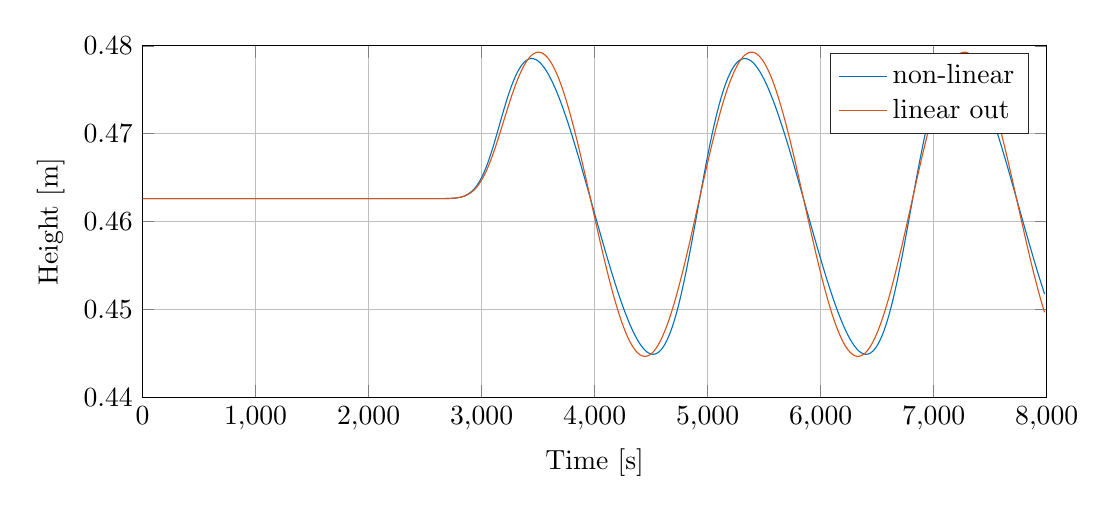
\begin{tikzpicture}

\begin{axis}[%
width=4.521in,
height=1.7566in,
at={(0.758in,0.481in)},
scale only axis,
xmin=0,
xmax=8000,
xlabel={Time [s]},
xmajorgrids,
ymin=0.44,
ymax=0.48,
ylabel={Height [m]},
ymajorgrids,
axis background/.style={fill=white},
legend style={legend cell align=left,align=left,draw=white!15!black}
]
\addplot [color=mycolor1,solid]
  table[row sep=crcr]{%
1	0.462595737606136\\
21	0.462595766861512\\
41	0.462595788438212\\
61	0.462595804181262\\
81	0.462595814989754\\
101	0.462595822807541\\
121	0.462595828630341\\
141	0.462595831905002\\
161	0.46259583412694\\
181	0.462595835844178\\
201	0.46259583699152\\
221	0.462595837729411\\
241	0.462595838185094\\
261	0.462595838461284\\
281	0.462595838623183\\
301	0.462595838711559\\
321	0.462595838750496\\
341	0.462595838752465\\
361	0.462595838721921\\
381	0.4625958386577\\
401	0.462595838554844\\
421	0.462595838406286\\
441	0.462595838204706\\
461	0.462595837944688\\
481	0.462595837625152\\
501	0.462595837251777\\
521	0.462595836838943\\
541	0.462595836410552\\
561	0.462595835999083\\
581	0.462595835642428\\
601	0.462595835378522\\
621	0.462595835238424\\
641	0.462595835239241\\
661	0.462595835378802\\
681	0.46259583563429\\
701	0.462595835965956\\
721	0.462595836326009\\
741	0.46259583667134\\
761	0.4625958369772\\
781	0.4625958372469\\
801	0.462595837510601\\
821	0.462595837811341\\
841	0.462595838185321\\
861	0.462595838646099\\
881	0.462595839178928\\
901	0.462595839745095\\
921	0.46259584029132\\
941	0.462595840759923\\
961	0.462595841098575\\
981	0.462595841269344\\
1001	0.462595841255849\\
1021	0.462595841066583\\
1041	0.462595840733295\\
1061	0.462595840304786\\
1081	0.462595839837555\\
1101	0.462595839385396\\
1121	0.462595838990585\\
1141	0.46259583867887\\
1161	0.462595838458964\\
1181	0.462595838325511\\
1201	0.462595838263768\\
1221	0.462595838254625\\
1241	0.46259583827901\\
1261	0.462595838320843\\
1281	0.462595838368157\\
1301	0.462595838412909\\
1321	0.462595838450395\\
1341	0.462595838478712\\
1361	0.462595838498255\\
1381	0.462595838511093\\
1401	0.462595838520255\\
1421	0.462595838528997\\
1441	0.46259583854018\\
1461	0.462595838555826\\
1481	0.462595838576902\\
1501	0.462595838603326\\
1521	0.462595838634151\\
1541	0.462595838667868\\
1561	0.462595838702734\\
1581	0.462595838737085\\
1601	0.462595838769557\\
1621	0.462595838799224\\
1641	0.462595838825622\\
1661	0.462595838848708\\
1681	0.462595838868759\\
1701	0.462595838886248\\
1721	0.462595838901721\\
1741	0.462595838915697\\
1761	0.462595838928591\\
1781	0.462595838940672\\
1801	0.462595838952052\\
1821	0.462595838962696\\
1841	0.462595838972448\\
1861	0.462595838981077\\
1881	0.462595838988318\\
1901	0.462595838993921\\
1921	0.462595838997697\\
1941	0.462595838999561\\
1961	0.462595838999575\\
1981	0.46259583899799\\
2001	0.462595838995287\\
2021	0.462595838992234\\
2041	0.462595838989955\\
2061	0.462595838990038\\
2081	0.462595838994679\\
2101	0.462595839006901\\
2121	0.462595839030852\\
2141	0.462595839072207\\
2161	0.46259583913876\\
2181	0.462595839241085\\
2201	0.462595839393452\\
2221	0.46259583961568\\
2241	0.462595839932888\\
2261	0.462595840379253\\
2281	0.462595841008547\\
2301	0.462595841858163\\
2321	0.462595843019391\\
2341	0.462595845638368\\
2361	0.4625958503106\\
2381	0.462595859125907\\
2401	0.462595874224808\\
2421	0.462595900568092\\
2441	0.46259594452641\\
2461	0.462596017209568\\
2481	0.462596133918965\\
2501	0.46259631785381\\
2521	0.462596599644938\\
2541	0.462597020085767\\
2561	0.462597629452957\\
2581	0.462598485211012\\
2601	0.462599653291652\\
2621	0.462601211614999\\
2641	0.462603270910744\\
2661	0.462606029337465\\
2681	0.462609870904031\\
2701	0.462615503569196\\
2721	0.462624112607928\\
2741	0.46263746573282\\
2761	0.462657927696744\\
2781	0.462688381305962\\
2801	0.462732126967519\\
2821	0.462792864345572\\
2841	0.462874800132007\\
2861	0.462982841012624\\
2881	0.463122751733321\\
2901	0.463301164887028\\
2921	0.463525383693851\\
2941	0.46380298787616\\
2961	0.464141275319514\\
2981	0.464546603824099\\
3001	0.465023723738187\\
3021	0.465575183944166\\
3041	0.466200875608223\\
3061	0.46689772826717\\
3081	0.467659571541626\\
3101	0.468477192712524\\
3121	0.469338619310273\\
3141	0.470229627253143\\
3161	0.471134437404302\\
3181	0.472036545221497\\
3201	0.472919622001497\\
3221	0.473768403009473\\
3241	0.474569438513391\\
3261	0.475311578027022\\
3281	0.475986128991952\\
3301	0.476586746354644\\
3321	0.477109177892581\\
3341	0.477550972074841\\
3361	0.477911178826543\\
3381	0.478190045081274\\
3401	0.478388723973582\\
3421	0.478509035502311\\
3441	0.478553294684254\\
3461	0.478524182145815\\
3481	0.478424623537686\\
3501	0.478257655473047\\
3521	0.478026314785805\\
3541	0.477733602173121\\
3561	0.47738254089049\\
3581	0.476976268333965\\
3601	0.476518060397594\\
3621	0.476011245130712\\
3641	0.47545904309026\\
3661	0.474864444741386\\
3681	0.474230207689763\\
3701	0.473558971311616\\
3721	0.472853408563272\\
3741	0.472116313052822\\
3761	0.471350571701492\\
3781	0.470559055223807\\
3801	0.469744502902326\\
3821	0.46890945975873\\
3841	0.468056279308506\\
3861	0.467187177240587\\
3881	0.466304314240948\\
3901	0.465409881535387\\
3921	0.464506158709552\\
3941	0.463595522263966\\
3961	0.462680405309402\\
3981	0.461763228435224\\
4001	0.460846328385924\\
4021	0.459931908983245\\
4041	0.459022034624202\\
4061	0.458118676734636\\
4081	0.457223800806582\\
4101	0.456339455804367\\
4121	0.455467824654186\\
4141	0.454611226317651\\
4161	0.453772100251186\\
4181	0.452953008380687\\
4201	0.452156648696482\\
4221	0.451385836185714\\
4241	0.450643426029038\\
4261	0.449932219537888\\
4281	0.449254929113725\\
4301	0.448614234014938\\
4321	0.448012878569118\\
4341	0.447453739908417\\
4361	0.446939839558729\\
4381	0.44647434512201\\
4401	0.446060595554607\\
4421	0.445702133914107\\
4441	0.445402706742644\\
4461	0.445166217376767\\
4481	0.444996657184716\\
4501	0.444898049706583\\
4521	0.444874383117409\\
4541	0.44492951658114\\
4561	0.445067050035481\\
4581	0.445290221202826\\
4601	0.445601871076422\\
4621	0.446004444523707\\
4641	0.446499957370417\\
4661	0.447089881838418\\
4681	0.447774969484852\\
4701	0.448555042272362\\
4721	0.449428783250223\\
4741	0.450393554823214\\
4761	0.45144526123565\\
4781	0.452578251837083\\
4801	0.453785262092848\\
4821	0.455057437346058\\
4841	0.456384522015529\\
4861	0.457755226755352\\
4881	0.459157658479834\\
4901	0.460579627094341\\
4921	0.462008752073201\\
4941	0.463432475906272\\
4961	0.464838171688495\\
4981	0.466213456263541\\
5001	0.467546667482304\\
5021	0.468827352513423\\
5041	0.470046586556222\\
5061	0.471197030174627\\
5081	0.472272770363773\\
5101	0.47326907833629\\
5121	0.474182212148699\\
5141	0.475009326281446\\
5161	0.475748486206027\\
5181	0.476398737917896\\
5201	0.476960143226998\\
5221	0.477433691431886\\
5241	0.477821069930187\\
5261	0.478124357961283\\
5281	0.478345765912584\\
5301	0.478487512168895\\
5321	0.478551852779087\\
5341	0.478541225105437\\
5361	0.478458394214516\\
5381	0.478306501319248\\
5401	0.478088959216268\\
5421	0.477809253818152\\
5441	0.477470786118439\\
5461	0.477076832102931\\
5481	0.47663058647073\\
5501	0.476135203510236\\
5521	0.475593780336078\\
5541	0.475009322157177\\
5561	0.474384750282148\\
5581	0.473722950736162\\
5601	0.473026799430022\\
5621	0.472299112843751\\
5641	0.471542551269154\\
5661	0.470759559127656\\
5681	0.469952405277727\\
5701	0.469123311086455\\
5721	0.46827459196725\\
5741	0.467408727973271\\
5761	0.466528318390822\\
5781	0.465635944291262\\
5801	0.464734028972795\\
5821	0.463824799057408\\
5841	0.462910378851767\\
5861	0.461992942586901\\
5881	0.46107480193166\\
5901	0.460158366463992\\
5921	0.459246018746161\\
5941	0.458339996203401\\
5961	0.457442349924919\\
5981	0.456555007564153\\
6001	0.455679931876339\\
6021	0.454819317892116\\
6041	0.453975716454362\\
6061	0.453151976708548\\
6081	0.452351008301765\\
6101	0.451575506849199\\
6121	0.45082783219231\\
6141	0.45011012604789\\
6161	0.44942459097568\\
6181	0.448773759457978\\
6201	0.448160613471587\\
6221	0.447588521960639\\
6241	0.447061063222956\\
6261	0.446581841206566\\
6281	0.446154386327256\\
6301	0.445782158282598\\
6321	0.445468610966842\\
6341	0.445217263297646\\
6361	0.445031741841928\\
6381	0.444915805522321\\
6401	0.444873351165655\\
6421	0.444908375095223\\
6441	0.445024827615758\\
6461	0.445226374670698\\
6481	0.44551615481219\\
6501	0.445896648950466\\
6521	0.446369693538927\\
6541	0.446936551429178\\
6561	0.447597931288157\\
6581	0.448353893073814\\
6601	0.449203647859668\\
6621	0.450145285496265\\
6641	0.451175466306077\\
6661	0.452289145414588\\
6681	0.453479432844087\\
6701	0.454737664462013\\
6721	0.456053668294621\\
6741	0.457416125332722\\
6761	0.458812927152067\\
6781	0.460231491336431\\
6801	0.46165905732883\\
6821	0.463082994401577\\
6841	0.464491098548183\\
6861	0.465871807792967\\
6881	0.467214296420706\\
6901	0.468508496672756\\
6921	0.469745148426169\\
6941	0.470915920459634\\
6961	0.472013588267787\\
6981	0.473032219475206\\
7001	0.473967322860057\\
7021	0.47481590339856\\
7041	0.475576347428661\\
7061	0.476248121577524\\
7081	0.476831397634691\\
7101	0.477326787330237\\
7121	0.477735296963816\\
7141	0.478058431459727\\
7161	0.478298287415192\\
7181	0.478457505420165\\
7201	0.478539068078455\\
7221	0.478546037683092\\
7241	0.478481356255522\\
7261	0.478347811075521\\
7281	0.47814814757116\\
7301	0.477885233336003\\
7321	0.477562154680077\\
7341	0.47718219234894\\
7361	0.476748713890495\\
7381	0.476265061745663\\
7401	0.475734478814768\\
7421	0.475160074919235\\
7441	0.474544828462544\\
7461	0.473891618610476\\
7481	0.473203272704271\\
7501	0.472482591551528\\
7521	0.47173231978675\\
7541	0.470955075285571\\
7561	0.470153299337239\\
7581	0.469329283635555\\
7601	0.468485269260669\\
7621	0.46762355399642\\
7641	0.46674654299248\\
7661	0.465856729240419\\
7681	0.464956638572598\\
7701	0.464048776136871\\
7721	0.46313558283631\\
7741	0.462219395731453\\
7761	0.461302419061183\\
7781	0.460386724760111\\
7801	0.459474291527016\\
7821	0.458567071551398\\
7841	0.457667064714051\\
7861	0.456776382674666\\
7881	0.4558972891119\\
7901	0.455032205739806\\
7921	0.454183683091857\\
7941	0.453354349456739\\
7961	0.452546859370056\\
7981	0.451763857819755\\
};
\addlegendentry{non-linear};

\addplot [color=mycolor2,solid]
  table[row sep=crcr]{%
1	0.462595737606136\\
21	0.462595737606136\\
41	0.462595737606136\\
61	0.462595737606136\\
81	0.462595737606136\\
101	0.462595737606136\\
121	0.462595737606136\\
141	0.462595737606136\\
161	0.462595737606136\\
181	0.462595737606136\\
201	0.462595737606136\\
221	0.462595737606136\\
241	0.462595737606136\\
261	0.462595737606136\\
281	0.462595737606136\\
301	0.462595737606136\\
321	0.462595737606136\\
341	0.462595737606136\\
361	0.462595737606136\\
381	0.462595737606136\\
401	0.462595737606136\\
421	0.462595737606136\\
441	0.462595737606136\\
461	0.462595737606136\\
481	0.462595737606136\\
501	0.462595737606136\\
521	0.462595737606136\\
541	0.462595737606136\\
561	0.462595737606136\\
581	0.462595737606136\\
601	0.462595737606136\\
621	0.462595737606136\\
641	0.462595737606136\\
661	0.462595737606136\\
681	0.462595737606136\\
701	0.462595737606136\\
721	0.462595737606136\\
741	0.462595737606136\\
761	0.462595737606136\\
781	0.462595737606136\\
801	0.462595737606136\\
821	0.462595737606136\\
841	0.462595737606136\\
861	0.462595737606136\\
881	0.462595737606136\\
901	0.462595737606136\\
921	0.462595737606136\\
941	0.462595737606136\\
961	0.462595737606136\\
981	0.462595737606136\\
1001	0.462595737606136\\
1021	0.462595737606136\\
1041	0.462595737606136\\
1061	0.462595737606136\\
1081	0.462595737606136\\
1101	0.462595737606136\\
1121	0.462595737606136\\
1141	0.462595737606136\\
1161	0.462595737606136\\
1181	0.462595737606136\\
1201	0.462595737606136\\
1221	0.462595737606136\\
1241	0.462595737606136\\
1261	0.462595737606136\\
1281	0.462595737606136\\
1301	0.462595737606136\\
1321	0.462595737606136\\
1341	0.462595737606136\\
1361	0.462595737606136\\
1381	0.462595737606136\\
1401	0.462595737606136\\
1421	0.462595737606136\\
1441	0.462595737606136\\
1461	0.462595737606136\\
1481	0.462595737606136\\
1501	0.462595737606136\\
1521	0.462595737606136\\
1541	0.462595737606136\\
1561	0.462595737606136\\
1581	0.462595737606136\\
1601	0.462595737606136\\
1621	0.462595737606136\\
1641	0.462595737606136\\
1661	0.462595737606136\\
1681	0.462595737606136\\
1701	0.462595737606136\\
1721	0.462595737606136\\
1741	0.462595737606136\\
1761	0.462595737606136\\
1781	0.462595737606136\\
1801	0.462595737606136\\
1821	0.462595737606136\\
1841	0.462595737606136\\
1861	0.462595737606136\\
1881	0.462595737606136\\
1901	0.462595737606136\\
1921	0.462595737606136\\
1941	0.462595737606136\\
1961	0.462595737606136\\
1981	0.462595737606136\\
2001	0.462595737606136\\
2021	0.462595737606136\\
2041	0.462595737606137\\
2061	0.462595737606138\\
2081	0.462595737606143\\
2101	0.462595737606155\\
2121	0.462595737606185\\
2141	0.46259573760626\\
2161	0.462595737606442\\
2181	0.462595737606881\\
2201	0.462595737607915\\
2221	0.462595737610311\\
2241	0.462595737615764\\
2261	0.462595737627956\\
2281	0.462595737654733\\
2301	0.462595737712507\\
2321	0.462595737834964\\
2341	0.462595738089961\\
2361	0.462595738611605\\
2381	0.462595739659966\\
2401	0.462595741729845\\
2421	0.462595745744776\\
2441	0.462595753395649\\
2461	0.462595767718986\\
2481	0.46259579406274\\
2501	0.462595841663183\\
2521	0.462595926160661\\
2541	0.46259607351919\\
2561	0.462596325986425\\
2581	0.462596750931272\\
2601	0.462597453611603\\
2621	0.462598595125208\\
2641	0.462600416936953\\
2661	0.462603273389091\\
2681	0.462607673407811\\
2701	0.462614332126884\\
2721	0.462624232274053\\
2741	0.462638693851075\\
2761	0.462659448883477\\
2781	0.462688715905299\\
2801	0.462729266569813\\
2821	0.462784474648894\\
2841	0.462858336113408\\
2861	0.462955448443918\\
2881	0.463080938255977\\
2901	0.463240329068703\\
2921	0.463439345704039\\
2941	0.463683658163351\\
2961	0.463978575310206\\
2981	0.464328706373438\\
3001	0.46473761501669\\
3021	0.465207495286579\\
3041	0.465738900112641\\
3061	0.466330550555491\\
3081	0.466979247640297\\
3101	0.467679898990943\\
3121	0.468425660825992\\
3141	0.469208183838434\\
3161	0.470017940829825\\
3181	0.470844606270707\\
3201	0.471677454272659\\
3221	0.472505742144354\\
3241	0.473319051383251\\
3261	0.474107565612145\\
3281	0.474862274193669\\
3301	0.475575099532513\\
3321	0.476238954078418\\
3341	0.476847738850598\\
3361	0.47739629850329\\
3381	0.477880348625895\\
3401	0.478296389589548\\
3421	0.47864161850588\\
3441	0.478913847491583\\
3461	0.479111433077405\\
3481	0.479233218721608\\
3501	0.479278490232898\\
3521	0.479246942531599\\
3541	0.479138655495855\\
3561	0.478954076489315\\
3581	0.478694007363406\\
3601	0.478359594104554\\
3621	0.47795231772777\\
3641	0.477473985421703\\
3661	0.476926721285119\\
3681	0.476312956249171\\
3701	0.475635416959559\\
3721	0.474897113512448\\
3741	0.474101326013728\\
3761	0.473251589977429\\
3781	0.472351680606591\\
3801	0.47140559601645\\
3821	0.470417539470096\\
3841	0.46939190070374\\
3861	0.468333236423857\\
3881	0.467246250062632\\
3901	0.46613577088155\\
3921	0.46500673251596\\
3941	0.463864151055931\\
3961	0.462713102760771\\
3981	0.461558701506231\\
4001	0.460406076064587\\
4021	0.459260347318534\\
4041	0.45812660551014\\
4061	0.45700988762592\\
4081	0.455915155018524\\
4101	0.454847271364446\\
4121	0.453810981055686\\
4141	0.452810888121376\\
4161	0.451851435773001\\
4181	0.450936886664109\\
4201	0.450071303952199\\
4221	0.44925853324693\\
4241	0.448502185524851\\
4261	0.447805621086561\\
4281	0.44717193462757\\
4301	0.446603941489189\\
4321	0.446104165150538\\
4341	0.445674826017232\\
4361	0.445317831556572\\
4381	0.445034767823046\\
4401	0.444826892411812\\
4421	0.444695128871457\\
4441	0.444640062600852\\
4461	0.444661938248348\\
4481	0.444760658624848\\
4501	0.444935785135602\\
4521	0.445186539728794\\
4541	0.445511808352268\\
4561	0.445910145903041\\
4581	0.446379782647601\\
4601	0.446918632084476\\
4621	0.447524300214145\\
4641	0.448194096175091\\
4661	0.448925044198757\\
4681	0.449713896830289\\
4701	0.450557149356322\\
4721	0.451451055375714\\
4741	0.452391643444058\\
4761	0.453374734718002\\
4781	0.454395961521012\\
4801	0.45545078674808\\
4821	0.456534524023167\\
4841	0.457642358519826\\
4861	0.458769368352508\\
4881	0.459910546443511\\
4901	0.461060822768411\\
4921	0.462215086881164\\
4941	0.46336821061879\\
4961	0.464515070884764\\
4981	0.465650572409904\\
5001	0.466769670389626\\
5021	0.467867392896996\\
5041	0.468938862971997\\
5061	0.469979320288883\\
5081	0.470984142305344\\
5101	0.471948864799536\\
5121	0.472869201703713\\
5141	0.473741064146368\\
5161	0.474560578618265\\
5181	0.475324104181655\\
5201	0.476028248646237\\
5221	0.476669883639971\\
5241	0.477246158507807\\
5261	0.477754512976569\\
5281	0.478192688529737\\
5301	0.478558738441577\\
5321	0.478851036426055\\
5341	0.479068283862095\\
5361	0.479209515563092\\
5381	0.479274104065045\\
5401	0.479261762414245\\
5421	0.479172545442164\\
5441	0.479006849521838\\
5461	0.478765410806871\\
5481	0.478449301960847\\
5501	0.478059927391703\\
5521	0.47759901701223\\
5541	0.477068618554415\\
5561	0.476471088471782\\
5581	0.475809081470146\\
5601	0.475085538713283\\
5621	0.474303674755941\\
5641	0.473466963262213\\
5661	0.472579121572749\\
5681	0.471644094189362\\
5701	0.470666035250401\\
5721	0.469649290074747\\
5741	0.468598375856442\\
5761	0.4675179615957\\
5781	0.466412847355485\\
5801	0.465287942935794\\
5821	0.464148246060404\\
5841	0.462998820172995\\
5861	0.461844771941289\\
5881	0.460691228569151\\
5901	0.459543315017457\\
5921	0.458406131234925\\
5941	0.457284729500069\\
5961	0.456184091974945\\
5981	0.455109108570406\\
6001	0.454064555221213\\
6021	0.453055072667523\\
6041	0.452085145837008\\
6061	0.451159083919233\\
6081	0.450281001220785\\
6101	0.449454798886248\\
6121	0.448684147566193\\
6141	0.447972471109226\\
6161	0.447322931350511\\
6181	0.446738414064377\\
6201	0.446221516143404\\
6221	0.44577453406095\\
6241	0.445399453668385\\
6261	0.44509794137235\\
6281	0.444871336731251\\
6301	0.44472064650387\\
6321	0.444646540176539\\
6341	0.444649346988744\\
6361	0.444729054470383\\
6381	0.44488530849717\\
6401	0.445117414863933\\
6421	0.445424342368832\\
6441	0.445804727394777\\
6461	0.446256879967709\\
6481	0.446778791264812\\
6501	0.447368142539305\\
6521	0.448022315422174\\
6541	0.448738403555052\\
6561	0.449513225502585\\
6581	0.450343338886913\\
6601	0.451225055681454\\
6621	0.452154458596072\\
6641	0.453127418480799\\
6661	0.454139612670824\\
6681	0.45518654419122\\
6701	0.456263561736095\\
6721	0.457365880333411\\
6741	0.45848860260365\\
6761	0.459626740517885\\
6781	0.460775237558584\\
6801	0.461928991184708\\
6821	0.463082875501263\\
6841	0.464231764032626\\
6861	0.46537055249844\\
6881	0.466494181490907\\
6901	0.467597658952714\\
6921	0.468676082355742\\
6941	0.469724660482008\\
6961	0.470738734710082\\
6981	0.471713799712407\\
7001	0.472645523471557\\
7021	0.473529766526521\\
7041	0.474362600363495\\
7061	0.475140324869477\\
7081	0.47585948477112\\
7101	0.476516884985823\\
7121	0.477109604816833\\
7141	0.477635010929317\\
7161	0.478090769049734\\
7181	0.478474854336547\\
7201	0.478785560376182\\
7221	0.479021506764281\\
7241	0.479181645238563\\
7261	0.479265264336037\\
7281	0.479271992553897\\
7301	0.479201800000023\\
7321	0.479054998525797\\
7341	0.478832240340602\\
7361	0.478534515114191\\
7381	0.478163145579783\\
7401	0.477719781657424\\
7421	0.477206393123726\\
7441	0.476625260860548\\
7461	0.475978966721493\\
7481	0.475270382061256\\
7501	0.474502654978772\\
7521	0.473679196330847\\
7541	0.472803664578406\\
7561	0.471879949532692\\
7581	0.470912155073615\\
7601	0.46990458091704\\
7621	0.468861703512017\\
7641	0.467788156152819\\
7661	0.466688708394148\\
7681	0.465568244860965\\
7701	0.464431743547083\\
7721	0.463284253698947\\
7741	0.462130873382844\\
7761	0.460976726835226\\
7781	0.459826941696755\\
7801	0.458686626231234\\
7821	0.457560846630612\\
7841	0.456454604506922\\
7861	0.455372814671118\\
7881	0.454320283297567\\
7901	0.453301686571179\\
7921	0.452321549912062\\
7941	0.451384227869991\\
7961	0.450493884778019\\
7981	0.449654476251187\\
};
\addlegendentry{linear out};

\end{axis}
\end{tikzpicture}%
\caption{Comparison of the nonlinear and linear model of the last pipe in the setup.}
\label{fig:linear_nonlinear_comparison_last_pipe}
\end{figure}

Here it start to have a small difference, which can be seen in the peaks of the figure. It seems as the nonlinear model starts to deviate from the linear model, as it rise faster and falls slower. However, it can be seen that the two model crosses in the operating point at each period and they still looks similar in phase and amplitude. The linear model, for small signal values is deemed to be a validate model for the nonlinear system and will be used in the next section in the design of an MPC controller. 

\section{Model predictive control}\label{se:model_predictive_control}
In this section, the design of the controller is elaborated. First the control problem the design of the Model predictive controller (MPC). 

The simulation covered in section ??? is to be controlled with respect to the problems elaborated in section \ref{sec:problem_statement} and stated here. 
\begin{enumerate}
\item Flow variations due to large industries and natural phenomenons
\item Concentration variations due to large industries and natural phenomenons
\begin{enumerate}
	\item Chloride variations
	\item Phosphor variations
	\item Nitrogen variations
	\item Organic matter variations
\end{enumerate}
\end{enumerate}

From the problem statement it is stated that flow and concentration variations must be kept to a minimum without causing any overflow in the sewer. To achieve this tanks are used, these are placed in the sewer network to find locations where they are able to hold back disturbance that will otherwise cause flow and concentration variations into the WWTP. However, the output of these tanks must be controlled in a way where overflow in the tank is prohibited. Therefore the controller must control the output of these tanks in an optimal manner to keep the input variations to the WWTP at a minimum and still be controlled according to some constraints.

To obtain such an optimal behavior MPC is chosen as stated in section \ref{sec:problem_statement}. MPC is an advanced control method which depends on a dynamic model of the system. Where the model, constraints and a cost function is used to generate the most optimal sequence of control inputs to the system, thus obtaining a desired process behavior. However, only the first control input is used in the current timeslot. Hereafter, in the next timeslot, the MPC algorithm is recalculated to find the must optimal input signal for this timeslot and so on. In addition, MPC also take future disturbance into account thereby predicting an output sequence that is optimal including the disturbance.  %The main advantage of MPC  Furthermore, MPC can be used with constraints to calculate the most optimal control output at the given timeslot and taking disturbance into the account. 
% In figure \ref{fig:control_of_sewer} it is shown that the MPC controller is setting the input to the pump.

% \begin{figure}[H]
% \centering
% \includegraphics[width=0.8\textwidth]{report/control/pictures/control_of_sewer.jpg}
% \caption{Block diagram of the system.}
% \label{fig:control_of_sewer}
% \end{figure}\fxnote{Der skal staa pumpe i stedet for tank}

% Where the iteration the in the MPC block can be described with the following items. 
% \begin{enumerate}
%        	\item Measurement is taken on the output if possible or it is taken directly from the states. If a state measurement is not available the state is estimated.
%        	\item Calculates a optimal set of predicted values over the prediction horizon according to a cost function and the constraints.
%        	\item The first element of the calculated control sequence is used as the control input.
%        	\item Repeat from 1.
% \end{enumerate}       

For MPC to optimize the system a cost function must be written to penalize variations of the flow output $Q(k+i|k)$ and the concentration output $C(k+i|k)$. Where k defines the time step and i is a value going from $1\leq H_p$, where $H_p$ is the prediction horizon. The cost function for flow and concentration is:

\begin{equation}
	 J = \sum_{i=1}^{H_p-1} || Q(k+i|k)C(k+i|k)-Q(k+i-1|k)C(k+i-1|k)||_{\CMcal{Q}(i)}^2
\end{equation}
Where J is the cost function that needs to be minimized, Q is the flow, C is the concentration and $\CMcal{Q}$ is a weighting parameter. It has been desired to only look at flow variation in the simulation and thereby excluding concentration from the cost function. This has been done to limit the control problem and ease the computation to begin with. Thereby the cost function has been rewritten to: 

\begin{equation}\label{eq:cost_function_height}
	 J = \sum_{i=1}^{H_p-1} || \hat{y}(k+i|k)-\hat{y}(k+i-1|k)||_{\CMcal{Q}(i)}^2
\end{equation}
\begin{equation}
	\begin{aligned}
	\text{s.t.} \hspace{5mm}  \hat{x}(k+i+1) &= A\hat{x}(k+i|k)+B\hat{u}(k+i|k)+B_dd(k+i|k) \\
						      \hat{y}(k+i)&= C\hat{x}(k+i|k) \\
						     \underline{\hat{x}} \leq \hat{x} \leq \overline{\hat{x}}
	\end{aligned}
\end{equation}
Where Q has been replaced with the output y as it can be measure directly from the state space system. y correspond to the height in the channel, however it is the same to minimize height difference as the flow because both describes the variation in the output of the sewer. In order for the controller to minimize the variations in the output it must be able to predicted future events from knowing the current state. Therefore, by iterating the linear model up to the prediction horizon the controller is able to predict future states. Thus by using the state equation recursively the state equation can be predicted up to the prediction horizon as shown in equation \ref{eq:iterating_state_equation}: 

\begin{equation}\label{eq:iterating_state_equation}
\begin{aligned}
	\hat{x}(k+1|k) &= A\hat{x}(k|k)+B\hat{u}(k|k) + B_dd(k|k)\\
	\hat{x}(k+2|k) &= A\hat{x}(k+1|k)+B\hat{u}(k+1|k)+ B_dd(k+1|k) \\
				   &= A^2\hat{x}(k|k)+AB\hat{u}(k|k)+AB_dd(k|k) + B\hat{u}(k+1|k) \\
				   &+ B_dd(k+1|k) \\
				   &\hspace{2mm}\vdots\\
   \hat{x}(k+H_p|k)&= A\hat{x}(k+H_p-1|k)+B\hat{u}(k+H_p-1|k)+B_dd(k+H_p-1|k)\\
   				   &= A^{H_p}\hat{x}(k|k)+A^{H_p-1}B\hat{u}(k|k)+A^{H_p-1}B_dd(k|k)+\hdots+\\
   				   &+B\hat{u}(k+H_p-1|k)+B_dd(k+H_p-1|k)
\end{aligned}
\end{equation}
Here the first equation $\hat{x}(k+1|k)$ is inserted into the second and this is iterated up to the prediction horizon. This can be setup as prediction vectors and matrices denoted by $\CMcal{X,A,B,U,B}_d$ and $\CMcal{D}$:


\begin{equation}\label{eq:lifted_state_equation}
\begin{aligned}
	  \underbrace{\begin{bmatrix}
	  \hat{x}(k+1|k) 	\\
	  \hat{x}(k+2|k) 	\\
	  \vdots 			\\
	  \hat{x}(k+H_p|k) 	\\
	   \end{bmatrix}}_{\CMcal{X}}
	 &=
	\underbrace{\begin{bmatrix}
		A \\
		A^2 \\
		\vdots \\
		A^{H_p} \\
	\end{bmatrix}}_{\CMcal{A}}
	\hat{x}(k|k) \\&+
	\underbrace{\begin{bmatrix}
		B 		 &0			 &\hdots	& 0		\\
		AB  	 &B  		 & \hdots& 0		\\
		\vdots 	 &\vdots	 & \ddots&\vdots	\\
		A^{H_p-1}B&A^{H_p-2}B&\hdots &B 
    \end{bmatrix}}_{\CMcal{B}}
    	\underbrace{\begin{bmatrix}
	\hat{u}(k|k)\\
	\hat{u}(k+1|k)\\
	\vdots\\
	\hat{u}(k+H_p-1|k)
	\end{bmatrix}}_{\CMcal{U}(k)} \\ &+ 
    \underbrace{\begin{bmatrix}
    	B_d 	    &0	         &\hdots & 0		\\
		AB_d  	    &B_d  	     & \hdots& 0		\\
		\vdots 	    &\vdots	     & \ddots&\vdots	\\
		A^{H_p-1}B_d&A^{H_p-2}B_d&\hdots &B_d 
 %   	B & \hdots & 0 \\
 %    	AB+B & \hdots & 0 \\
 %    	\vdots & \ddots & \vdots \\
 %    	\sum_{i=0}^{H_u-1}A^i B & \hdots & B \\
 %    	\sum_{i=0}^{H_u}A^i B & \hdots & AB+B\\
 %    	\vdots & \vdots & \vdots \\
 %    	\sum_{i=0}^{H_p-1}A^i B & \hdots & \sum_{i=0}^{H_p-H_u}A^i B \\
	  \end{bmatrix}}_{\CMcal{B}_d} 
	\underbrace{\begin{bmatrix}
	d(k|k)\\
	d(k+1|k)\\
	\vdots\\
	d(k+H_p-1|k)
	\end{bmatrix}}_{\CMcal{D}(k)}
	\end{aligned}
\end{equation}

Where $\CMcal{X}$ is the predicted state vector for the entire prediction horizon. $\CMcal{A}$ is the state matrix up to the prediction horizon. $x(k|k)$ is the initial state and is used to predict the hole prediction horizon, $\CMcal{B}$ is the input matrix for the prediction horizon, $\CMcal{U}$ is the predicted input vector, which consist of all the predicted inputs from the current timestep until $(k+H_p-1)$. $\CMcal{B}_d$ is the disturbance matrix for the prediction horizon and $\CMcal{D}$ is the disturbance vector. 

This iteration process is also done for the output equation:

\begin{equation}\label{eq:lifted_output_equation}
	\CMcal{Y}(k)= 
	\begin{bmatrix}
	y(k+1|k)\\
	y(k+2|k)\\
	\vdots\\
	y(k+H_p-1|k)
	\end{bmatrix}
	= 
	\underbrace{\begin{bmatrix}
	C 		& 0 	&\hdots	& 0\\
	0 		& C 	&\hdots & 0 \\
	\vdots	& \vdots&\ddots & 0\\
	0 		& 0		&0 		& C
	\end{bmatrix}}_{\CMcal{C}}
	  \underbrace{\begin{bmatrix}
	  \hat{x}(k+1|k) 	\\
	  \hat{x}(k+2|k) 	\\
	  \vdots 			\\
	  \hat{x}(k+H_p|k) 	\\
	   \end{bmatrix}}_{\CMcal{X}}
\end{equation}
Where $\CMcal{C}$ is a diagonal matrix with the output matrix C and $\CMcal{X}$ the predicted state vector. By inserting the predicted state equation \ref{eq:lifted_state_equation}, into the predicted output equation \ref{eq:lifted_output_equation} the following is achieved:

\begin{equation}\label{eq:output_eq_with_state_eq}
	\CMcal{Y}(k) =  \CMcal{C}\CMcal{A}x(k) +  \CMcal{C}\CMcal{B}\CMcal{U}(k) +\CMcal{C}\CMcal{B}_d\CMcal{D}(k)
\end{equation}   

By using the following notation on equation \ref{eq:output_eq_with_state_eq}:


\begin{equation}
 \psi = \CMcal{C}\CMcal{A}  \hspace{5mm} \gamma = \CMcal{C}\CMcal{B} \hspace{5mm}  \Theta = \CMcal{C}\CMcal{B}_{d}
\end{equation}

The predicted output equation can be rewritten as: 

\begin{equation}\label{eq:lifted_output_with_states_inserted}
	\CMcal{Y}(k) = \psi x(k) + \gamma \CMcal{U}(k) + \Theta \CMcal{D}(k)
\end{equation}

To be able to use the cost function, equation \ref{eq:cost_function_height}, it has to be rewritten so the predicted output equation can be used. This is done by replacing the output y with the predicted output $\CMcal{Y}$ thereby the following is obtained:

\begin{equation}
	J = ||\CMcal{Y}(k)-\CMcal{Y}(k-1)||_{\CMcal{Q}(i)}^2
\end{equation}
Where the difference between $\CMcal{Y}(k)$ and $\CMcal{Y}(k-1)$ can be expressed as:

\begin{equation}
	\Delta \CMcal{Y}(k) =\CMcal{Y}(k)-\CMcal{Y}(k-1) 
\end{equation}

Thereby the following cost function is achieved:

\begin{equation}\label{eq:delta_cost_function}
	J = \Delta\CMcal{Y}(k)^T \cdot Q \cdot \Delta\CMcal{Y}(k)
\end{equation}

To be able to write the cost function as quadric and linear terms of the predicted output $\Delta\CMcal{U}$, equation \ref{eq:lifted_output_with_states_inserted} is therefore inserted into equation \ref{eq:delta_cost_function} and thereby the following is obtained:

\begin{equation}
	J = (\psi\Delta x(k) + \gamma\Delta \CMcal{U}(k) + \Theta\Delta \CMcal{D}(k))^T\cdot Q \cdot (\psi\Delta x(k) + \gamma\Delta \CMcal{U}(k) + \Theta\Delta \CMcal{D}(k))
\end{equation}


\begin{equation}
	\begin{aligned}
	&(\psi\Delta x(k) + \gamma\Delta \CMcal{U}(k) + \Theta\Delta \CMcal{D}(k))^T\cdot Q \cdot (\psi\Delta x(k) + \gamma\Delta \CMcal{U}(k) + \Theta\Delta \CMcal{D}(k)) = \\
	& \Delta x(k)^T\psi ^T Q \psi \Delta x(k) 								+ \underbrace{\Delta x(k)^T \psi ^T Q \gamma \Delta  \CMcal{U}(k) }_{Linear}				+\Delta x(k)^T \psi ^T Q \Theta \Delta \CMcal{D}(k) \\
	& \underbrace{\Delta \CMcal{U}(k)^T \gamma ^T Q \psi\Delta x(k)}_{Linear} + \underbrace{\Delta \CMcal{U}(k)^T\gamma ^T Q \gamma\Delta \CMcal{U}(k)}_{Quadric} +\underbrace{\Delta \CMcal{U}(k)^T \gamma ^T Q\Theta \Delta \CMcal{D}(k)}_{Linear} \\ 
	& \Delta \CMcal{D}(k)^T \Theta ^T Q  \psi \Delta x(k)					+ \underbrace{\Delta \CMcal{D}(k)^T \Theta ^T Q \gamma  \Delta \CMcal{U}(k) }_{Linear}	+\Delta \CMcal{D}(k)^T \Theta ^T Q \Theta \Delta \CMcal{D}(k)
	\end{aligned}
\end{equation}



\begin{equation}
	\CMcal{H} = \gamma^T Q\gamma 
\end{equation}

\begin{equation}
	\begin{aligned}
	\CMcal{G} &= 2 \Delta x(k)^T\psi^T Q \gamma+2 \Delta \CMcal{D}(k)^T\Theta^T Q \gamma 
	\end{aligned}
\end{equation}

And a constant term that can be seen in appendix

\begin{equation}
	J = \Delta U(k)^T\CMcal{H}\Delta U(k)+ \CMcal{G}\Delta U(k)+ c
\end{equation}

The optimization is given by

\begin{equation}
	\min_{\Delta U(k)} J(\Delta U(k)) =\min_{\Delta U(k)} \Delta U(k)^T\CMcal{H}\Delta U(k)+\CMcal{G}\Delta U(k)+c
\end{equation}